
\chapter{Etapas propostas no Plano de Trabalho} \label{Etapas}
As etapas do \textit{Plano de Trabalho} buscou direcionar as atividades de pesquisa de modo que a cada passo fosse possível formar uma base sólida de entendimento da área de pesquisa. A fim de alcançar os objetivos do Projeto de Pesquisa as etapas a seguir foram estipuladas:
\begin{enumerate}
    \item  Estudo bibliográfico das perspectivas nacional e internacional no que diz respeito a veículos autônomos;
    \item  Pesquisa bibliográfica para compreender o que busca economicamente e tecnologicamente o mercado internacional e nacional em relação a veículos autônomos;
    \item Aprender quais são os diferentes tipos de veículos autônomos;
    \item Pesquisa bibliográfica das tecnologias essenciais de um carro autônomo;
    \item Mapear e entender os principais softwares de controle de um carro autônomo;
    \item Elaboração do Relatório Final.
\end{enumerate}

No decorrer desse ano de pesquisas foi possível desenvolver, de forma satisfatória, todas as etapas do projeto. Contudo, a etapa 5 devido a sua grandiosidade necessita de uma pesquisa única e mais aprofundada. De modo a aprofundar e consolidar os conhecimentos na área de software para a direção autônoma.

\newpage
\chapter{Objetivos} \label{Objetivos}
\section{Objetivo Geral}\label{Objetivo Geral}
Neste primeiro ano concluído, os nossos objetivos foram documentar e entender o cenário de Veículos Autônomos (VAs) no mundo e nesse processo contrastar com o brasileiro. De modo a compreender o cenário automobilístico e suas expectativas para essa categoria de veículos. Ademais, foi buscado identificar as principais diferenças entre esses veículos e o que se espera economicamente e tecnologicamente dessa tecnologia, tanto para o Brasil e o mundo. Por fim, mapeamos quais são os principais recursos tecnológicos que fazem esses veículos possíveis. Principal interesse neste projeto de pesquisa na área computacional. 

\section{Objetivos em Específico}\label{Objetivos Específicos}
\begin{enumerate}
    \item  Entender o cenário de Veículos Autônomos no mundo, e contrastar com o brasileiro:
    \begin{enumerate}
        \item Compreender o cenário automobilístico brasileiro, e as suas expectativas para essa tecnologia.
        \item Contrastar o mercado de veículos autônomos mundial com o brasileiro, buscando  decifrar o que é necessário para a aplicação dessa tecnologia no país.
    \end{enumerate}
    \item  Estudar as principais empresas de pesquisa que trabalham com Veículos Autônomos no mundo, e o que buscam economicamente e tecnologicamente no setor:
    \begin{enumerate}
        \item Identificar se buscam diferentes tipos de Carros Autônomos. Assim como entender as suas possíveis principais diferenças.
        \item Entender o que essas empresas buscam alcançar economicamente, e tecnologicamente ao inserir essa tecnologia no mercado.
        \item Conhecer as mudanças econômicas que carros autônomos podem trazer para a sociedade brasileira. 
    \end{enumerate}
    \item Mapear as tecnologias essenciais para a Direção Autônoma:
    \begin{enumerate}
        \item Documentar quais são os Softwares, algoritmos de controle, e sensores usados nesses veículos.  
    \end{enumerate}
\end{enumerate}

\newpage
\chapter{Metodologia} \label{Metodologia}
Utilizamos uma metodologia, com o propósito de revisar a literatura existente, que tem como essência desenvolver e colocar as pessoas envolvidas em contato direto com todo material já desenvolvido em relação a esta iniciação científica, constituída principalmente de: artigos científicos, cursos online, publicações em periódicos, jornais online, monografias e dissertações.

Nesse formato metodológico, pesquisa bibliográfica, foi possível ter contato e se fundamentar com os principais materiais da atualidade relacionados a veículos autônomos, de modo a ter contato com o que há de mais recente sobre o assunto.

Ressaltamos que, com o decorrer das pesquisas, foram encontradas fontes relevantes, que já possuem mais de 3 anos desde sua publicação. Devido a isso, tomamos essas publicações como ponto de partida para atualizar-se sobre o que há de mais novo sobre o assunto, de maneira a sempre manter o conteúdo deste relatório o mais atual possível.

A pesquisa bibliográfica seguiu as etapas ilutradas na Figura \ref{img_bibli}:

\begin{figure}[H]
\centering
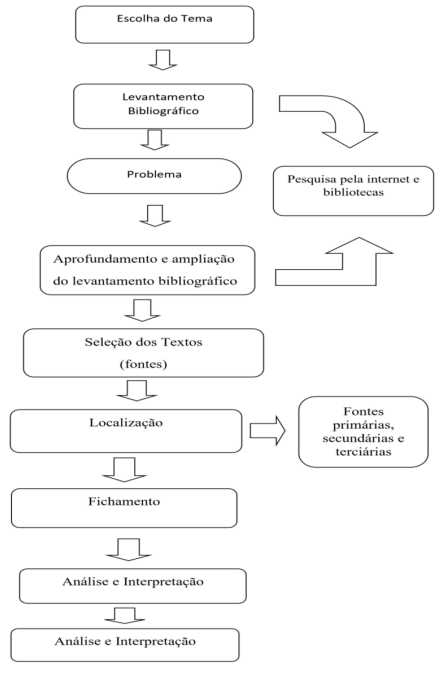
\includegraphics[width=8cm]{Figures/bibli.png}
\caption{Etapas da pesquisa Bibliográfica \cite{bibli}.}
\label{img_bibli}
\end{figure}

As etapas apresentadas na Figura \ref{img_bibli}, foram seguidas de modo a auxiliar na
delimitação do tema a ser pesquisado e em sua organização. Na sequencia, forneceremos detalhes de cada uma das etapas desenvolvidas neste projeto.
%\vspace {1cm}
%A seguir forneceremos detalhamento para as etapas (Figura \ref{img_bibli}) da pesquisa bibliográfica desenvolvida neste projeto:\vspace {1mm}
\begin{itemize}\label{details}

\item \textbf{Escolha do tema:} A escolha do tema foi feita no desenvolvimento do Plano de Trabalho para esta Iniciação Científica; Veículos Autônomos e suas tecnologias. 

\item \textbf{Levantamento Bibliográfico:} O levantamento preliminar foi feito através dos seguintes meios na internet (Google academic, Google livros, biblioteca virtual, bibliotecas, site das bibliotecas de universidades, CAPES e outros). Foram pesquisadas referências na plataforma \url{scholar.google.com}, no portal do Periódico CAPES, e jornais e artigos pela internet. A busca nos bancos de dados abrangeu principalmente os anos de 2020 a 2023. Contudo, a partir de pesquisas na internet, também, fizemos uso de materiais publicados a partir de 2018 devido as suas melhores definições e maior relevância. Como palavra-chave utilizou-se os termos: \textit{Autonomous Vehicles}, \textit{Autonomous, Cars, Mobility, Connected Car, AV, TaxiBot}, e \textit{self-driving cars}.  %A pesquisa limitou-se aos idiomas inglês, português,  alemão, e espanhol (ordenado por maior uso).


\item \textbf{O problema:} Devido ao enquadramento dessa pesquisa, por visar unicamente o enriquecimento dos conhecimentos sobre os materiais já desenvolvidos sobre o tema. Este trabalho não busca responder, necessariamente, a um problema de pesquisa. Devido a isso, podemos enquadrar nossos Objetivos (seção \ref{Objetivos}) nessa etapa, de modo a ser nossa estrela guia para desenvolver a pesquisa.

\item \textbf{Aprofundamento e ampliação do levantamento bibliográfico:} Buscamos por obras (artigos, teses, matérias) mais recentes, dos últimos 3 anos, para nos mantermos atualizados evitando conteúdos obsoletos. Mantivemos um número razoável de fontes bibliográficas, de modo a não nós perdermos durante o desenvolvimento da pesquisa. 

\item \textbf{Seleção das fontes:} Houve a seleção das fontes mais relevantes para o projeto a partir de filtros: o primeiro filtro ocorreu pela leitura dos seus títulos, sendo selecionados os que se referiam as palavras-chave apresentadas no \textit{Levantamento Bibliográfico}. A segunda filtragem foi realizada a partir da leitura dos resumos. Neste filtro foi possível identificar publicações que apresentaram relevância para o nosso tema.
Portanto, por meio de uma leitura crítica buscamos assimilar as obras levantadas, sempre analisando se faria sentido usá-las para o desenvolvimento do projeto. 

\item \textbf{Localização das fontes:} Como apresentado na etapa de  \textit{Levantamento Bibliográfico} fizemos uso de recursos online para este projeto. Sobretudo, da plataforma CAPES.

\item \textbf{Fichamento:} Para este projeto não foi realizada a classificação dos artigos encontrados. Entretanto, nessa etapa, foram feitos resumos e rascunhos de modo a auxiliar no firmamento dos conhecimentos, e no desenvolvimento do relatório final.

\item \textbf{Análise e Interpretação:} Buscamos averiguar se os materiais encontrados contém valor teórico para o projeto, se sofreu alterações, interpolações, e possíveis falsificações ao longo do tempo. Houve, também, a checagem das fontes dos materiais apresentados, de modo a sempre buscar pela fonte principal do assunto, e nos principais meios de mídias globais.


\end{itemize}

 
Como apresentado no plano de trabalho, a Iniciação Científica buscou seguir um princípio metodológico \textit{“Project-based learning”}\footnote{Aprendizagem baseada em projetos} \cite{krajcik2006project}, que visa construir soluções a partir de problemas reais em nossa sociedade. Visto que, é uma modalidade de estudo que deixa as pessoas envolvidas livres para seguir a sua curiosidade, desejo de resolver os problemas encontrados pelo caminho e de buscar por mais informações para resolvê-los. Contemplando assim os objetivos desejados para a realização de maneira satisfatória deste projeto. 

Além disso, as pesquisas realizadas são fundamentadas no método de pesquisa \textit{Revisão Sistemática de Literatura} (RSL) que segundo Maria Cristiane (Universidade de São Paulo) \cite{revi3}, e Davi Nakano (Universidade de São Paulo) \cite{revi2} refere-se a um tipo de investigação que se concentra em uma questão bem definida, visando identificar, selecionar, avaliar e sintetizar as evidências disponíveis relacionadas a uma questão formulada de interesse para o pesquisador, esse princípio e método foram utilizados nas etapas definidas na Figura \ref{img_bibli}.

Por fim, enaltecemos que devido ao formato de pesquisa, as fontes foram crescendo com o passar do tempo. Portanto, o levantamento bibliográfico encontra-se muito mais rico comparado com o início da seleção bibliográfica.


\vspace {0,5cm}

Utilizamos, também, os seguintes formatos de aprendizado durante o desenvolvimento do projeto:
\begin{itemize}
\item \textit{Cursos e minicursos;}
\item \textit{Participação em eventos.}
\end{itemize}
Como pode ser observado na seção \ref{eventos}
\newpage

\chapter{Resultados e Discussão} \label{resultados}

Os resultados deste primeiro ano de pesquisa são desenvolvidos nas próximas seções e subseções. A ordem de apresentação dos resultados segue o que foi proposto nos \textit{Objetivos} definidos no Capítulo \ref{Objetivos}. Desse modo, desenvolvemos cada objetivo proposto, elaborando e apresentando os resultados e conclusões das pesquisas, mais recentes, encontradas sobre o assunto.

\section{Veículos Autônomos no Brasil e no mundo}

Nesta seção tratamos do potencial transformativo dos VAs, focamos em pesquisas que nos trouxeram tendências, benefícios, e problemas para implementação de VAs no Brasil e no mundo. No aspecto de implementação, foi possível identificar setores da sociedade em que VAs podem ser amplamente utilizados e áreas em que já são aplicados na atualidade. Ademais, durante as pesquisas, foram encontrados relatórios e artigos que nos trouxeram uma visão analítica do cenário de VAs para 30 países do mundo, nos enriquecendo com dados concretos sobre o cenário atual para essa categoria de veículos. 

\subsection{Implementação de Veículos Autônomos no Brasil e no Mundo}

Antes de entendermos como implementar VAs, precisamos entender quais veículos são esses: Veículos autônomos são todos os veículos que não exigem um motorista humano de maneira parcial ou total para conduzi-los, ou seja, veículos que podem se dirigir sozinhos. Alguns veículos que podem ser considerados autônomos já fazem parte do cotidiano de certas cidades, são os metrôs e trens que não precisam de motorista, ou o motorista só está ali para casos extremos. No entanto, devido aos últimos avanços e inovações tecnológicas, a automação de conduções está se expandindo para muitas categorias de veículos como: caminhões, ônibus, escavadeiras (entre outros veículos industriais), e até barcos, navios e aviões. Devido a automação desses meios de transporte, o mundo experimentará reviravoltas sem precedentes por conta do potencial transformativo dos VAs \cite{4cenarios_ocidental}.

Diante disso, o estudo de sua implementação, a ser desenvolvido nos próximos subcapítulos, é fundamental para compreendermos quais âmbitos da nossa sociedade essa categoria de veículos podem ser alocados, e os benefícios e dificuldades de sua implementação no Brasil e no mundo.

 \subsubsection{Expectativas com a implementação dos Veículos Autônomos}
Devido ao seu potencial transformativo, vários benefícios são esperados. Entre esses benefícios e expectativas estão o de redução de acidentes de trânsito. Estimou-se que no brasil o número de mortes em acidentes de transporte terrestre no período de 2019 foi de 31.945 \cite{Anexo_I_pnatrans}. Veículos autônomos vêm com a promessa de buscar uma redução nesses números através da retirada do principal causador de acidentes de trânsito: erros humanos. 

Ademais, Veículos Autônomos vem como uma forma de minimizar os congestionamentos nas grandes metrópoles. Segundo o  Plano Estratégico de Desenvolvimento Urbano Integrado da Região Metropolitana do Rio de Janeiro, \cite{rj_transito}, apenas na hora do \textit{rush} da manhã o fluxo de viagens de São Gonçalo a Niterói chega a quase 100 mil pessoas sendo transportadas; desses deslocamentos cerca de 80\% das viagens são feitas em transporte público, ônibus convencionais. 

Diante disso, uma das propostas para suprir essa demanda de transporte seria a inclusão de veículos autônomos. Nesse formato, carros poderiam ser solicitados como, hoje, são feitas as corridas de aplicativos, e os ônibus do transporte público  poderiam operar por mais horas e com menor custo \cite{4cenarios_ocidental}. 
Entretanto, ainda seria necessário lidar com problemas como: a disputa de espaço nas vias, e os engarrafamentos crônicos das cidades. Por exemplo, de acordo com informações do levantamento domiciliar realizado durante a elaboração do último Plano Diretor de Transporte Urbano (PDTU), o tempo médio de deslocamento do centro de São Gonçalo a Niterói é de 50 minutos, devido a problemas relacionados ao grande fluxo de veículos, sendo no transporte público o tempo gasto de quase 25\% maior \cite{rj_transito}.


No sentido de solucionar problemas como o exemplificado, um estudo de caso considerando um cenário onde veículos autônomos têm que lidar com congestionamentos, levou à conclusão de que o aumento do número de veículos autônomos, totalmente conectados dirigindo em pelotões dentro de uma rede, reduz os atrasos e congestionamentos, como visto na Figura \ref{congestionamento}. 

\begin{figure}[H]
\centering
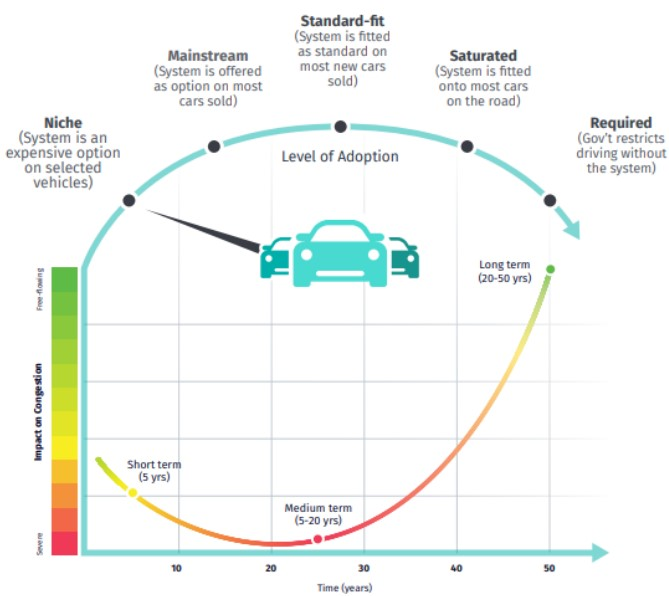
\includegraphics[width=15cm]{Figures/conge.jpg}
\caption{Impacto dos níveis de autonomia no congestionamento ao longo do tempo \cite{4cenarios_ocidental}.}
\label{congestionamento}
\end{figure}
\begin{quote}
Descrição da figura \ref{congestionamento}: Eixo y: cor vermelha (parte debaixo da barra na esquerda da figura) exemplifica que os VAs estão contribuindo para o congestionamento, e a cor verde (parte superior da barra na esquerda da figura) representa o outro lado do espectro de cor, logo, representando, a diminuição ou não contribuição no congestionamento. Eixo x: Tempo (anos)

\end{quote}

No estudo, os VAs mantiveram ou melhoraram o tráfego da rota escolhida. Isso foi possível pois, o veículo líder do pelotão foi capaz de antecipar mudanças nos sinais e comunicá-las com os veículos de trás, permitindo um melhor desempenho em cruzamentos sinalizados \cite{conge}.

A seguir, na Figura \ref{mapa_resumo}, apresentamos um mapa da visão geral dos benefícios, riscos e mudanças incertas com a aplicação dos VAs na sociedade, de modo a termos uma ideia do que esperar dessa categoria de veículos:

\begin{figure}[H]
\centering
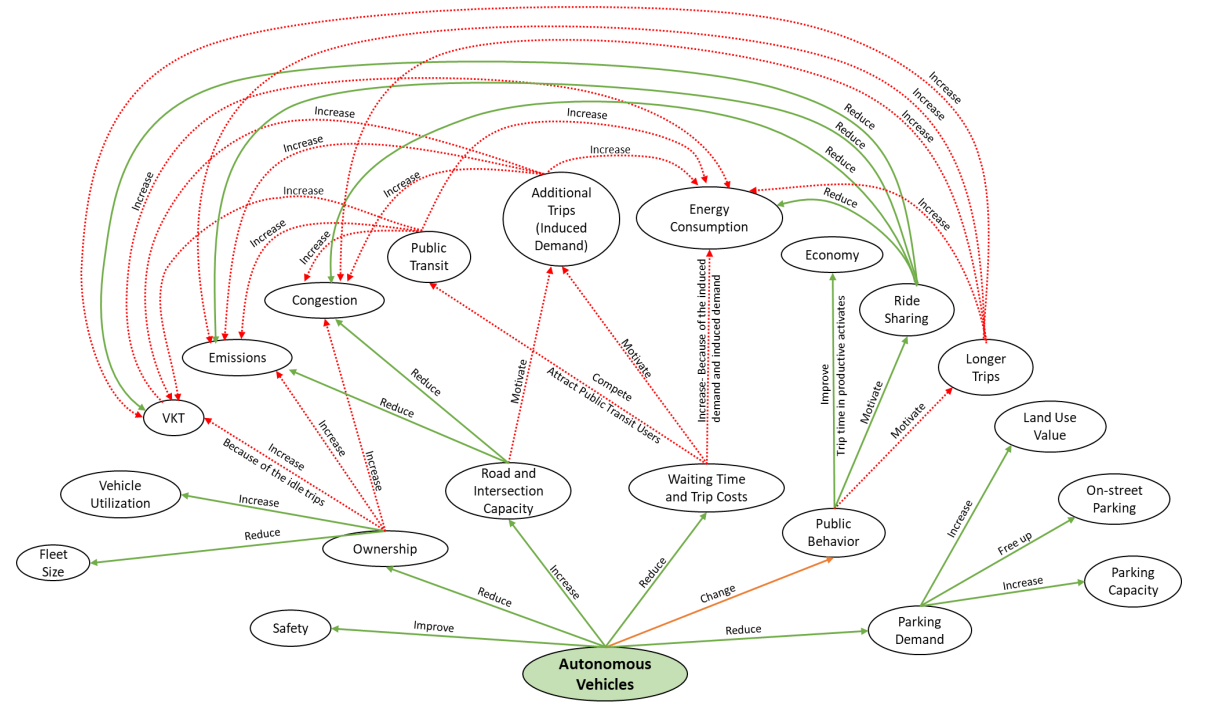
\includegraphics[width=16cm]{Figures/map.png}
\caption{Mapeando a relação entrelaçada entre as implicações dos VAs (verde = benefício, vermelho = risco, laranja = mudança incerta) \cite{mundobrasil}.}
\label{mapa_resumo}
\end{figure}


\subsubsubsection{Implementação em setores industriais} \label{industria}

Ainda tratando sobre os benefícios de VAs em nossa sociedade. Nos deparamos com a utilidade dessa categoria em ambiente industrial, onde podem operar em indústrias automotivas, de bebidas, eletroeletrônicos, suplementos agrícolas, portos, linhas de montagem, etc.

Dentre essas utilidades, temos a aplicação de veículos autônomos em portos. Cujo é uma aplicação que visa aumentar a eficiência do transporte de contêineres e materiais para os navios e setores do próprio porto. O uso desses veículos aumenta a automação da movimentação logística, acelerando o processo de carga, descarga e armazenamento.
Portanto, isso faz com que a produção tenha um ganho significativo, através do aumento da produtividade e redução dos custos. Pois essas máquinas podem atuar de maneira ótima em rotas programadas tanto na função de abastecimento das linhas de produção, quanto na transferência entre estações ou áreas do processo produtivo, e no transporte de matéria-prima ou produto acabado \cite{aplicacao}.

\subsubsection{Veículo Autônomo e áreas de implementação} \label{implementacao}

Devido a sua simplicidade, segurança e conforto em operação. Os VAs podem ser aplicados em diversas áreas e setores da sociedade como, na execução de funções e tarefas de risco que seres humanos não seriam capazes de realizar, ou na execução de funções exaustivas onde o ser humano teria uma menor eficiência. Visto que a maioria desses veículos têm suas funções executadas automaticamente, necessitando de nenhum ou pouca supervisão de um humano. Desse modo, se tornam perfeitos, também, para pessoas com necessidades específicas e idosos pois os VAs poderam auxiliar essas pessoas no seu dia a dia, fazendo com que essas pessoas vivam uma vida de forma mais independente. 
\vspace {1cm}

A seguir apresentaremos aplicações especializadas de Veículos Autônomos \cite{aplicacao2}:

\begin{enumerate}
 \item \textbf{Transporte público:} Veículo Autônomos foram introduzidos inicialmente no sistema de transporte público na modalidade de operação sem condutor. Hoje em dia, essas tendências modernas no transporte público são úteis e trazem benefícios nas região metropolitana para os turistas e os próprios cidadãos. Como mencionado anteriormente, um dos benefícios do trânsito sem motorista seria melhorar o serviço para passageiros com algum tipo de necessidade específica. O serviço de transporte para pessoas com necessidade específica, geralmente, é inconveniente, não confiável e caro. Em algumas cidades os passageiros com algum tipo de necessidade específica \ref{implementacao}, normalmente, precisam reservar uma viagem 24 horas antes da partida e são informados de que a coleta pode ocorrer a qualquer momento durante uma janela de 2 horas \cite{notif}. Desse modo, os VAs vêm como uma possível melhoria no estilo de vida de muitas pessoas.
\item \textbf{Bonde e Trem Elétrico Autônomo:} O primeiro veículo sobre trilhos elétrico automatizado foi projetado e desenvolvido pela Siemens na Alemanha, e em 2018, o primeiro \textit{Test Drive} do bonde foi realizado por sete quilômetros. O uso de dispositivos inteligentes, como câmeras, sensores e sistemas LiDAR (apresentados na Figura \ref{figura-sensores}) baseados em software, são úteis para o Bonde dirigir em áreas lotadas de várias cidades. Devido ao algoritmo inteligente, sistemas de monitoramento e controle, um Bonde operará com segurança mesmo nessas áreas com muito tráfego de pessoas e veículos, e diante de qualquer obstáculos, o bonde se encarregará de solucionar a situação com o auxílio de recursos auxiliares, e iniciará o trajeto imediatamente após a retirada do obstáculo do seu caminho. Um exemplo similar de Bonde, foi o Harry projetado e desenvolvido em 2017, na Inglaterra. Visando suprir a falta de transporte público em algumas localidades de Londres.
\item \textbf{Helicóptero Elétrico Autônomo:} O VSR700 é um dos protótipos inovadores de Helicópteros Elétricos Autônomos inventados em 2020 pela Airbus e testado na França. Esses veículos foram projetados e desenvolvidos para operar ao lado de vários meios navais. O objetivo é dar suporte aos navios, aumentando seu escopo fazendo uso de sensores inteligentes, de modo a aprimorar o cenário de coleta de informações para os navios. Esses Helicópteros Autônomos estão fazendo o trabalho de vigilância das informações de seus alvos e confirmando o destino de chegada das embarcações. 
\item \textbf{Caminhão Inteligente Autônomo:} Um caminhão elétrico totalmente automatizado foi projetado e desenvolvido em 2016 com o nome Otto. Sem motorista humano, opera com a ajuda do sistema LiDAR (visto \ref{figura-sensores}). Esses caminhões modernos minimizam os acidentes e são utilizados para entrega de mercadorias e serviços pesados. Além disso, o caminhão elétrico autônomo Vera, um Volvo, foi projetado e desenvolvido para transportar mercadorias de diversos destinos, como indústrias, estaleiros, minas, portos, pátios de armazenamento e armazéns. Sendo muito mais eficiente, segura, limpo e sustentável do que os caminhões atuais mais comuns.

\item \textbf{Veículos Subaquáticos Autônomos:} São usados em estudos geográficos da marinha e também são populares no setor técnico e de defesa. A principal função destes veículos é obter uma imagem aprimorada do fundo do mar com uma resolução muito alta, e da estrutura de uma embarcação no mar, ou qualquer objeto sobre investigação.
\item \textbf{Veículos Autônomos para Agricultura e Mineração:}  Os VAs, também, são aplicados em vários processos no setor agrícola, mineração de mesmo modo como apresentado nas tarefas operacionais de portos \ref{industria}. Os diferentes tipos de VAs aplicados para a agricultura e mineração são: tratores agrícolas autônomos, caminhões de mineração inteligentes, máquinas automatizadas de mineração, etc.

\end{enumerate}

Ainda na perspectiva de implementação, os VAs podem ser introduzidos no âmbito de veículos de entrega, transporte público, e em um contexto de pandemia na detecção de infectados, como apresenta a Figura \ref{resumo_aplic}:

\begin{figure}[H]
\centering
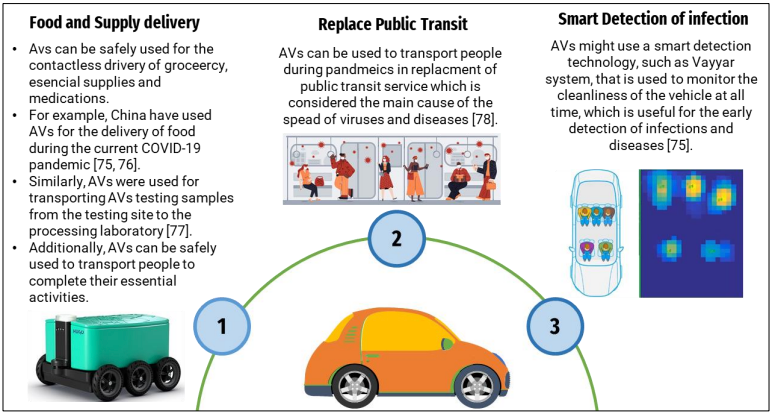
\includegraphics[width=\textwidth]{Figures/aplic.png}
\caption{Resumo dos benefícios dos VAs e aplicações \cite{mundobrasil}.}
\label{resumo_aplic}
\end{figure}

\begin{quote}

A Figura \ref{resumo_aplic} apresenta um resumo de 3 aplicações de utilização dos VAs e seus respectivos beneficios. Na sequência fizemos uma breve descrição para um melhor entendimento:

\begin{enumerate}
 \item \textbf{Entrega de suplementos e comidas:} Apresentando que os VAs podem ser uma alternativa segura e útil para a entrega de medicamentos, suplementos essenciais, produtos de supermercado. Como exemplo prático, a figura introduz o uso dessas VAs na China durante a pandemia de COVID-19 no transporte de suplementos de modo geral. Assim como, o uso em laboratório no transporte de material em teste, e no transporte de pessoas.

\item \textbf{Transporte público:} Apresenta, também, que os VAs são uma excelente alternativa para o transporte da população. 

\item \textbf{Detecção de infectados:} Por fim, os VAs podem ser equipados de tecnologias capazes de detectar e monitorar pessoas infectadas no veículo, ou identificar se o VA está sujo e precisando de algum tipo de manutenção. 

\end{enumerate}

\end{quote}

\subsection{O cenário de aplicação de Veículos Autônomos}
Segundo o relatório, “2020 Autonomous Vehicles Readiness Index” da \cite{KPMG}; empresa que opera em 143 países e territórios em todo o mundo, oferecendo serviços de auditoria, impostos e consultoria.
Que buscou avaliar a preparação de 30 países e jurisdições, apresentado na Figura \ref{KPMG}, fazendo uso de um índice composto que combina 28 medidas individuais de uma variedade de fontes em uma única pontuação. Tudo isso, visando ser uma relatório para ajudar a medir o nível de preparação para essa categoria de veículos pelo mundo. Mais informações sobre os resultados, metodologias e fontes utilizadas no relatório podem ser encontradas em, \cite{KPMG}.

\begin{figure}[H]
\centering
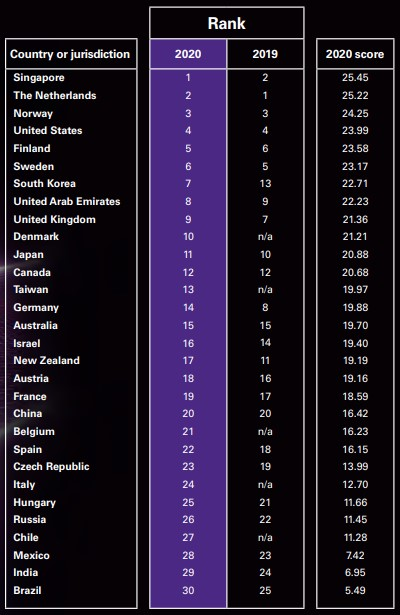
\includegraphics[width=8cm]{Figures/rank.jpg}
\caption{Resultado do relatório 2020 Autonomous Vehicles Readiness Index \cite{KPMG}.}
\label{KPMG}
\end{figure}

Observando o Ranking\footnote{Uma posição em uma escala de conquista ou status; uma classificação.} \ref{KPMG} notamos que o Brasil, entre os países estudados, encontra-se na trigésima posição, ficando na última colocação. Dentre os pilares citados e estudados pela KPMG o Brasil apenas não ficou em último lugar na questão de aceitação do consumidor, apresentado na Figura \ref{rank30}, ficando na vigésima nona posição.
Entre os pontos apresentados, o estudo ressalta que o governo brasileira está fazendo muito pouco para encorajar a adoção dos VAs, assim refletindo na última posição do ranking. Por outro lado, o país tem entusiasmo por novas tecnologias e serviços, como carona. Diante disso, o chefe de governo da KPMG no Brasil e na América do Sul, Maurício Endo, diz:
\begin{quote}
    
“Ainda não vemos nenhuma política pública para criar um caminho para que os VAs comecem a operar nas cidades do Brasil”.
\end{quote}

\begin{figure}[H]
\centering
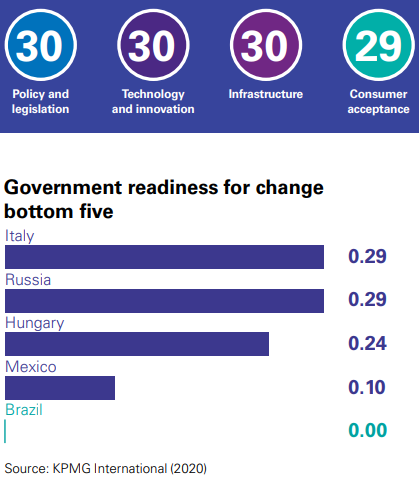
\includegraphics[width=8cm]{Figures/rank30.png}
\caption{Posição do Brasil no relatório \cite{KPMG}.}
\label{rank30}
\end{figure}

Por outro lado, nessa perspectiva de pavimentar o caminho para a operação de VAs nas cidades brasileiras, surge o programa Rota 2030, lançado em 2018, que ofereceu incentivos para substituir os tipos de motores tradicionais por híbridos ou Veículos Elétricos. De mesmo modo, em Outubro de 2019 houve o lançamento de uma pequena frota de carros elétricos Renault Twizy junto com pontos de recarga em Brasília, permitindo que funcionários públicos se descolassem entre prédios do governo de maneira mais econômica e com menos emissões de carbono do que antes.

Ademais, em janeiro de 2020, a montadora brasileira de veículos Hitech Electric lançou o que chamou de primeiro VA desenvolvido no país. O e.coTech4 elétrico de dois lugares, que pode atingir velocidades de 50 km/h, está inicialmente disponível apenas para aluguel corporativo em áreas fechadas, como áreas industriais, campus universitários e resorts \cite{KPMG}.


Ainda tratando sobre as perspectivas do VAs, temos o estudo anual da indústria do \textit{Connected Car Innovation} (CCI) que formulou um índex que busca pesquisar empiricamente e comparar o desempenho e a força inovadora de 28 fabricantes globais de automóveis nas áreas de veículos e serviços conectados, bem como sua força de mercado usando vários indicadores. O estudo é baseado no banco de dados de inovação do Centro de Gestão Automotiva (CAM) \cite{CCI}. A partir deste estudo, podemos identificar, como mostra a Figura \ref{forcaCCI}, que o Brasil não encontra-se como uma força inovadora nas áreas de arquitetura veicular, conectividade/infoentretenimento e direção autônoma dos \textit{players}\footnote{Um participante significativo.} mais importantes do universo dos carros conectados.


\begin{figure}[H]
\centering
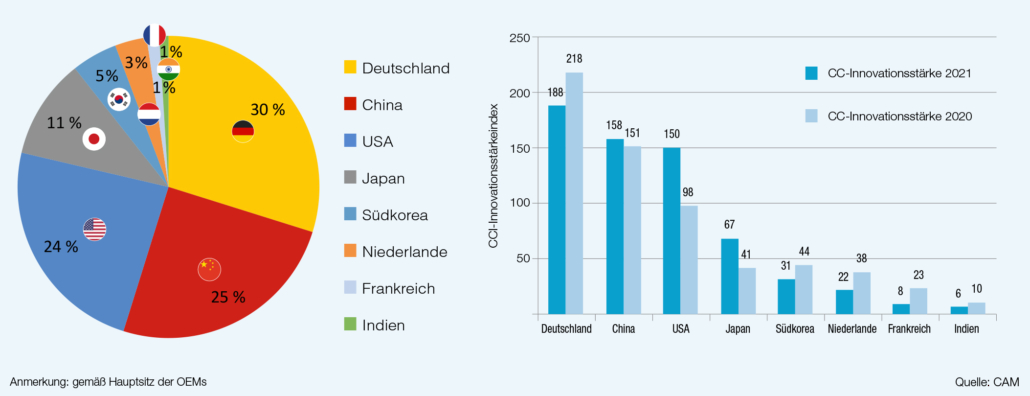
\includegraphics[width=12cm]{Figures/CCI.jpg}
\caption{Força inovadora por país  \cite{CCI}.}
\label{forcaCCI}
\end{figure}


Diante de tudo isso, apesar do pouco encorajamento do governo brasileiro quanto a adoração de veículos autônomos, e a baixa aceitação do Brasil comparado com os demais países da lista. Ainda precisamos tratar sobre questões relacionadas à infraestrutura do país para a navegação e operação desses veículos. 
O principal problema que os VAs enfrentarão são os sistemas de sinalização e marcação precários, gerenciamento de tráfego ruim em caso de incidência de trânsito, e heterogeneidade do tráfego \cite{mundobrasil}.

As Figuras \ref{awareness} e \ref{public} mostram um mapa detalhado dessas principais barreiras e suas implicações nos VAs pelo mundo.
\begin{figure}[H]
\centering
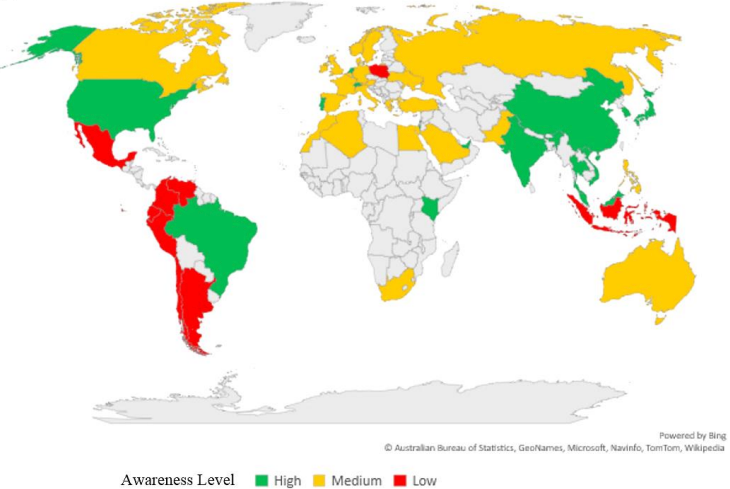
\includegraphics[width=12cm]{Figures/grafik-a.png}
\caption{Resumo do nível de consciência em diferentes países com diferentes níveis de PIB \cite{mundobrasil}, variando de Alto (verde), Médio (amarelo) e Baixo (vermelho).}
\label{awareness}
\end{figure}

\begin{figure}[H]
\centering
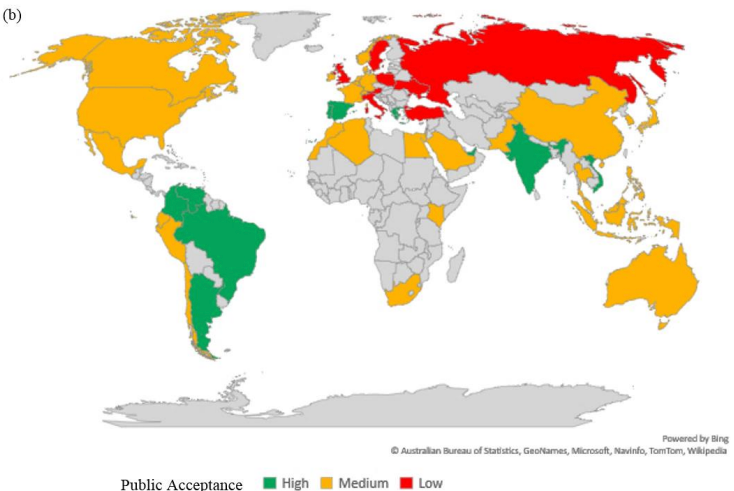
\includegraphics[width=12cm]{Figures/grafik-b.png}
\caption{Resumo do nível de aceitação pública em relação aos VAs em diferentes países com diferentes níveis de PIB \cite{mundobrasil}, variando de Alto (verde), Médio (amarelo) e Baixo (vermelho).}
\label{public}
\end{figure}

É possível identificar nas Figuras \ref{awareness} e \ref{public} que o Brasil encontra-se com um nível alto em consciência e aceitação do público. Para mais detalhes da análise dos principais desafios para a navegação segura de VAs em países em desenvolvimento, \cite{mundobrasil}.

Ainda mais, nos artigos levantados, também, podemos identificar que o Brasil têm melhores pontos no quesito infraestrutura comparada com os outros pontos analisados, e, entretanto, ainda se encontra muito atrás comparado com os outros países analisados.

\begin{figure}[H]
\centering
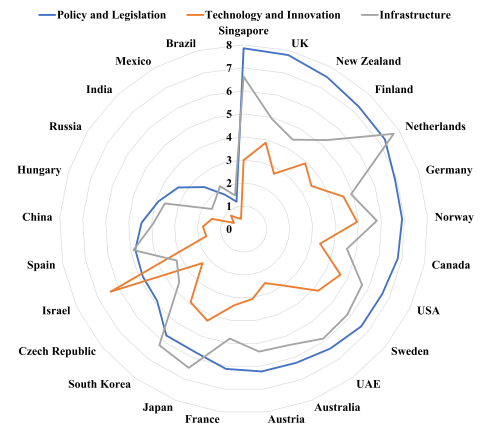
\includegraphics[width=8cm]{Figures/future.png}
\caption{Os sucessos alcançados pelos 25 principais países até agora em relação aos VAs em termos de política, legislação, tecnologia, inovação e infraestrutura \cite{future-view}.}
\label{figura_future-view}
\end{figure}



Por fim, como identificado nas Figuras \ref{rank30} e \ref{figura_future-view}, Singapura foi a localidade com maior aproveitamento somando os pilares estudados pelo \textit{Autonomous Vehicles Readiness Index 2020} \cite{KPMG}, tendo em vista os esforços adicionais que tem feito para encorajar o uso de VAs. Em janeiro de 2019, o governo da cidade e estado publicou seu rascunho de padrões, TR68, para esses veículos, bem como uma estrutura voluntária de governança de IA \cite{KPMG}. A KPMG relata que desde o primeiro relatório publicado os países têm apresentado rápidas e fortes mudanças a caminho da implementação e da ampliação das frotas de veículos autônomos, no desenvolvimento de regularizações e incentivos, além de que a mídia começou a considerar as vantagens e desvantagens dos VAs, as empresas testam cada vez mais veículos e por consequência os consumidores estão aceitando a ideia de migração para Veículos Autônomos, e o Brasil, apesar das suas tentativas em 2018 e 2020 ainda tem, como apresentado, uma longa estrada com pouca sinalização e baixa infraestrutura para percorrer de modo a permitir o uso de VAs em maiores proporções no país.

\newpage
\section{Veículos Autônomos e suas perspectivas}

Nesta seção tratamos sobre as perspectivas dos VAs em nossas sociedades, identificamos quais são os diferentes tipos de VAs e apresentamos a sua taxonomia\footnote{Processo que descreve a diversidade dos seres vivos, feito usando artifícios como a classificação e nomenclatura.} com base em fontes reconhecidas mundialmente. Buscamos fazer essa apresentação de maneira bem didática e de forma ilustrativa para uma melhor compreensão de todos. Ademais, trouxemos um panorama de como encontra-se o mercado tecnológico e econômico para os VAs; quais são as principais empresas que trabalham e pesquisam nessa categoria de veículos, e quais são as expectativas de lucro de algumas dessas empresas.

\subsection{Nível de condução autônoma}  \label{nv3}
	
Na busca de identificar os diferentes tipos de Carro Autônomos, nos deparamos com um cenário ainda em processo de definição. Pois, com os presentes avanços na área de veículos autônomos, surgiu a necessidade das empresas e dos órgãos de regularização, de classificá-los de alguma forma. Desse modo, a \textit{Society of Automotive Engineers} (SAE), uma das principais associações globais que busca essa classificação, como apresentado nas Figuras \ref{Graph_PT} e \ref{Graph_EN}, dividiu os veículos autônomos em seis níveis de funcionalidade, que vão desde nenhum recurso de automação (nível 0) até automação completa, sem a necessidade de um condutor humano, (nível 5). Fazendo uso da terminologia “sistemas de direção autônoma” para se referir a veículos que possuem algum tipo de direção autônoma \cite{SAE}. Nesse cenário, os níveis 1 e 2 incluem alguns recursos, enquanto o nível 3 alcança automação limitada, onde o motorista pode abrir mão do controle do veículo, desde que esteja disponível para intervir quando solicitado.

Abaixo, Figuras \ref{Graph_PT} e \ref{Graph_EN}, apresentamos graficamente as diferenças de Veículos Autônomos e suas respectivas classificações \cite{SAE}:

\begin{figure}[H]
\centering
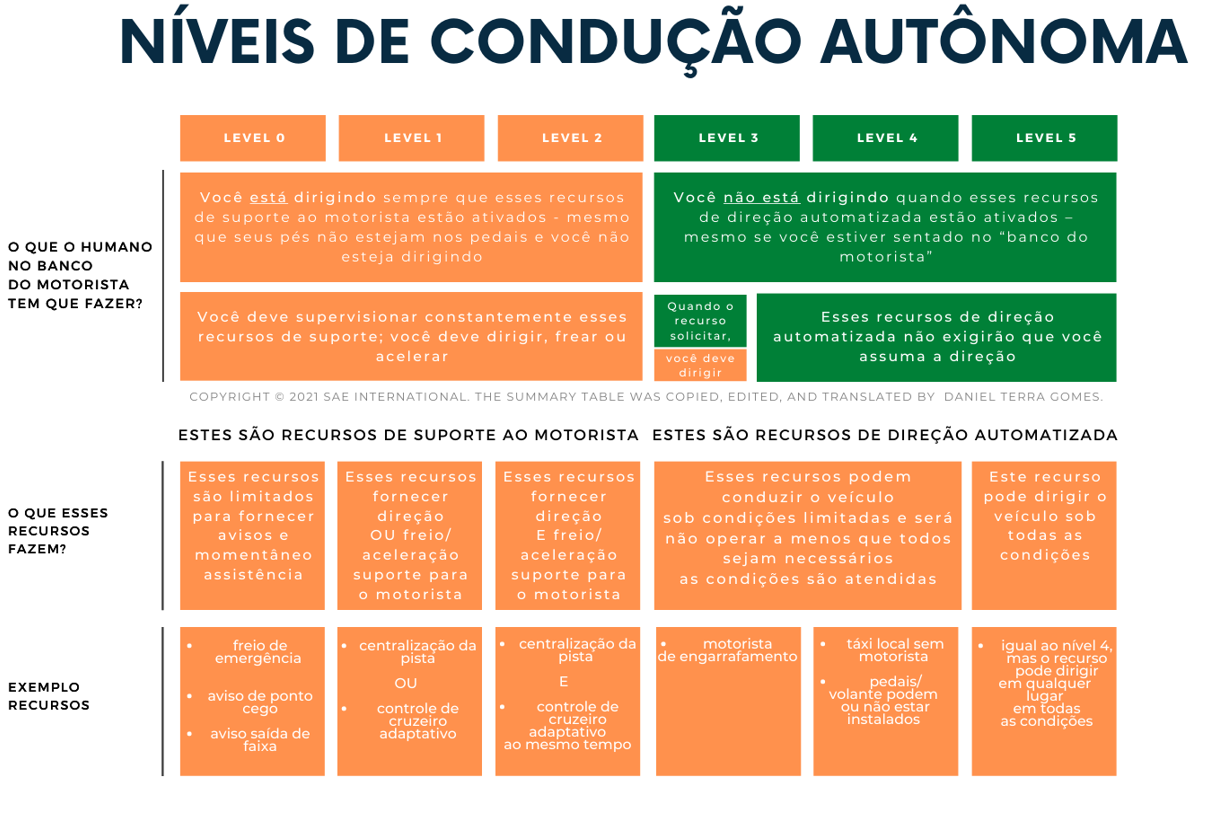
\includegraphics[width=15cm]{Figures/IC-Graph1.png}
\caption{Níveis de Automação de condução PT-BR}
\label{Graph_PT}
\end{figure}
\begin{figure}[H]
\centering
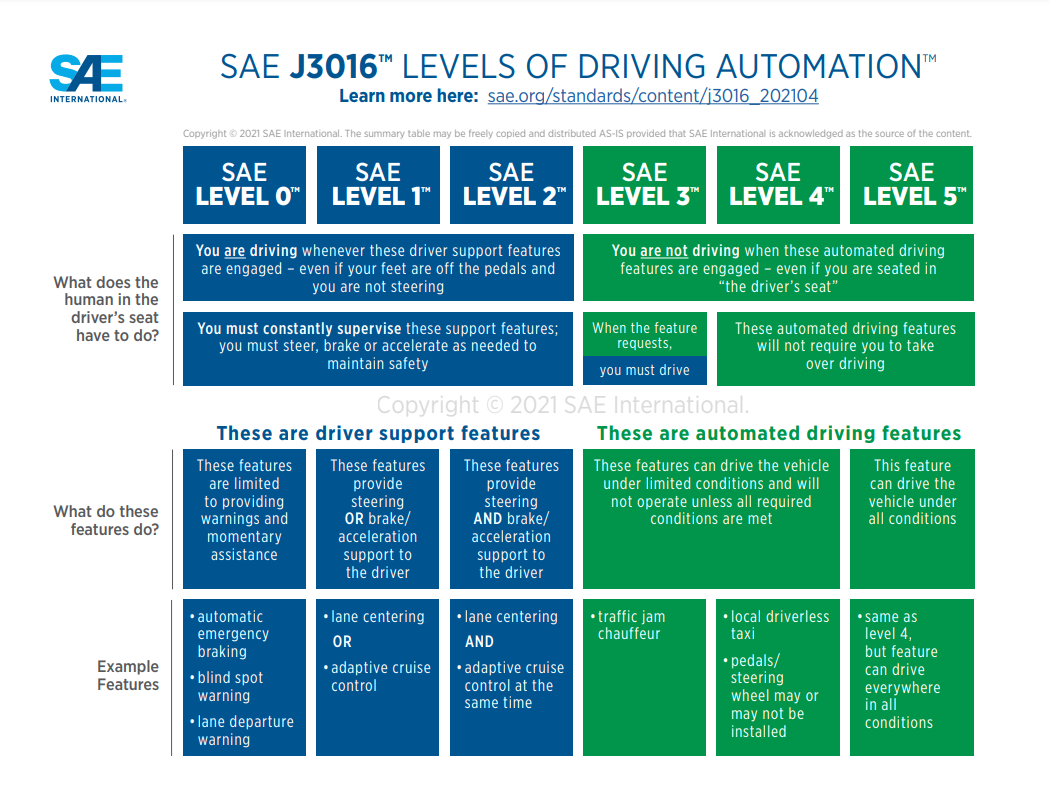
\includegraphics[width=15cm]{Figures/IC-GrapEN.png}
\caption{SAE J3016TM levels of driving automation \cite{SAE}}
\label{Graph_EN}
\end{figure}

Além dessas classificações entre tipos veículos, ainda é possível classificá-los nas seguintes categorias de tipos de automação: Sistema de Assistência Avançada ao Motorista (ADAS) sigla do inglês \textit{advanced driver-assistance system (ADAS)}, ou Condução Automática, Mobilidade Como Serviço (MaaS) sigla do inglês \textit{Mobility as a service (MaaS)}.
Como apresentado, nas Figuras \ref{Graph_PT} e \ref{Graph_EN}, nos níveis 1, 2 e 3 o condutor precisa estar preparado para caso o sistema precise de algum tipo de ajuda do condutor, esses níveis são vistos como uma espécie de remendo, pois funcionam como um ajudante para suprir uma demanda que os sistemas autônomos, como um todo, ainda não podem cumprir com maestria \cite{4cenarios_ocidental}. Dado que o objetivo com o avanço da tecnologia é que o condutor humano torna-se cada vez menos necessário, e como apresentado no nível 5, Figura \ref{Graph_EN}, é possível até mesmo a retirada do volante do veículo. 

Na atualidade, empresas líderes do setor de veículos autônomos, como a Tesla, ainda trabalham com nível 2 de direção autônoma referente ao ADAS para veículos vendidos para a população. \cite{4cenarios_ocidental}.
Por outro lado, no início do ano de 2023, a Mercedes-Benz, no seu portal de mídias, afirma ser a primeira empresa a alcançar a marca de direção autônoma SAE level 3 para o mercado dos Estados Unidos, sendo o estado de Nevada o primeiro a concordar com as regulamentações para a navegação desses tipos de veículos em seu território. A Mercedes afirma, também, que já em 2024 terá os seus primeiros veículos \textit{DRIVE PILOT}, em portugues “condutor”, disponíveis para o mercado Norte Americano \cite{mercedes3}.

\begin{quote}
“No mundo moderno, o tempo é um dos bens mais preciosos, e devolver o tempo aos nossos clientes é um elemento central em nossa estratégia de construir os carros mais desejados do mundo. O nosso DRIVE PILOT dá um grande passo para o conseguir e coloca-nos na vanguarda da inovação no campo crucialmente importante da condução autónoma. O DRIVE PILOT demonstra mais uma vez que nosso pioneirismo faz parte do nosso DNA. A certificação em Nevada marca o início de seu lançamento internacional e, com ela, o início de uma nova era.”

\end{quote}
Diz o Markus Schäfer, Membro do Conselho de Administração do Mercedes‑Benz Group AG, Diretor de Tecnologia, responsável por Desenvolvimento e Compras \cite{mercedes3}.

Adicionalmente, algumas empresas, como Waymo e Cruise, atualmente operam serviços de carona com veículos com autonomia de nível 4 nos Estados Unidos da América (EUA) - isso significa que os carros podem operar sem motorista ao volante sob certas condições, como dentro de uma área de serviço designada, portanto, já mapeadas e entendida pelo algoritmo e software de controle dos veículos \cite{Houser2023-dn}.



A seguir forneceremos as definições detalhadas para seis níveis de automação de veículos, variando de nenhuma automação de direção (Nível 0) a automação total de direção (Nível 5), no contexto de veículos a motor, definidos pela SAE \cite{SAE}:

\begin{enumerate} \label{SAE-level}
 \item \textbf{Nível 0} – Sem automação de condução: Não existe nenhum tipo de auxílio ao motorista e nenhuma presença/atuação de tecnologia de condução autônoma, ou assistência.

\item \textbf{Nível 1} - Assistência ao Motorista: No nível 1, o motorista é assistido apenas em relação à velocidade do veículo, um exemplo prático seria o piloto automático, que mantém a velocidade do veículo constante de acordo com o gosto do motorista. Neste caso, o condutor deve continuar a frear, acelerar e direcionar o veículo. Um segundo exemplo seria: o recurso de assistência ao estacionamento, executa automaticamente as ações de controle de movimento do veículo necessárias para estacionar um veículo, enquanto o motorista executa as ações de controle de movimento do veículo longitudinal e supervisiona o recurso de estacionamento.

\item \textbf{Nível 2} - Automação de Condução parcial: Nesta fase, o veículo já é capaz de realizar ações de forma autônoma, como frear, acelerar e parar o veículo em uma direção, como é o caso da tecnologia chamada ACC (Adaptive Cruise Control). No nível 2, o condutor continua a ser responsável pela condução e exige que o condutor esteja atento à condução e retome a condução em situações de perigo. Um exemplo prático seria, como visto: o recurso de assistência ao estacionamento, mas dessa vez, executa automaticamente as ações de controle de movimento lateral e longitudinal do veículo necessárias para estacionar um veículo sob a supervisão do motorista.

\item \textbf{Nível 3} - Automação Condicional de Condução: Consiste em veículos que são capazes de se mover de forma independente, tanto na direção, aceleração e frenagem. Neste nível de condução, o condutor pode realizar outras atividades enquanto o carro segue autonomamente a sua rota, mas por vezes é acionado para assumir a condução por um curto período de tempo ou para assumir o controlo total em situações de risco. Nesse cenário, um \textit{automated driving system} (ADS)  é capaz de continuar a executar o \textit{dynamic driving task} (DDT) por pelo menos vários segundos após fornecer ao usuário pronto para \textit{fallback}\footnote{Um plano de backup ou estratégia de contingência; uma alternativa que pode ser usada se algo der errado com o plano principal; um recurso.}; uma solicitação para intervir. Espera-se então que o usuário pronto para o \textit{fallback} do DDT retome a operação manual do veículo ou alcance uma condição de risco mínimo se ele/ela/elu determinar que é necessário.

\item \textbf{Nível 4} - Alta Automação de Condução: O veículo controla todas as tarefas 
que antes eram do condutor, sem necessidade da atenção do mesmo. Desse modo, o veículo fica encargo de executar todo o DDT em uma localidade, ao sofrer uma falha de sistema relevante para o desempenho do DDT. Em resposta, o \textit{ADS-dedicated vehicle} (ADS-DV) realiza o \textit{fallback} do DDT ligando os piscas de emergência, manobrando o veículo para o acostamento e estacionando-o, antes de chamar automaticamente a assistência de emergência. Nesse  nível, o ADS é capaz de atingir automaticamente uma condição de risco mínimo quando necessário.

\item \textbf{Nível 5} - Automação de Condução completa: permite que o veículo elimine a necessidade de um motorista humano, com todos os controles e tarefas de direção realizados por um sistema autônomo. O desempenho do veículo é sustentado, incondicionalmente, por um ADS responsável por todo o DDT e \textit{fallback} do DDT sem qualquer expectativa de que um usuário precise intervir.

\end{enumerate}

A Figura \ref{niveis-auto} é a representação didática de todos os diferentes níveis (0-5) de autonomia SAE \ref{SAE-level} já discutidas nesse relatório:

\begin{figure}[H]
\centering
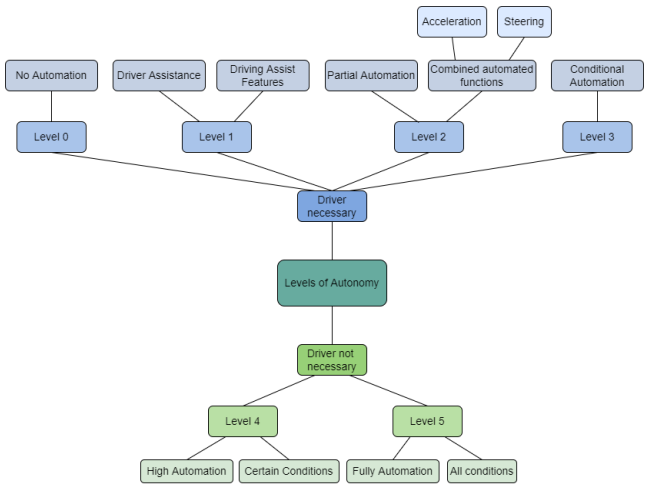
\includegraphics[width=\textwidth]{Figures/level-auto.png}
\caption{Níveis de Autonomia \cite{review-auto}.}
\label{niveis-auto}
\end{figure}

\begin{quote}
Descrição da figura \ref{niveis-auto}:  \textit{Nível 0} - Sem automação.  \textit{Nível 1} - Assistência ao motorista e funcionalidades de assistência.  \textit{Nível 2} - Automação parcial e funcionalidades de assistência combinadas.  \textit{Nível 3} - Automação condicionada.  \textit{Nível 4} - Alta automação em certas condições.  \textit{Nível 5} - Totalmente autônomo em todas as condições. 
\end{quote}



\subsection{Condução Autônoma e mercado tecnológico}

A inserção da Condução Autônoma no mercado dependerá da demanda de viagens por veículos, da infraestrutura de transporte, do grau de automação desses veículos, da taxa na qual os veículos autônomos são introduzidos no mercado, e da confiança da sociedade com essa categoria de transporte. 

Como visto, na Figura \ref{Graph_EN} os níveis de automação de 0 a 3 exigirão a presença de um motorista no veículo. O nível 4 a 5, não fazem a exigência de ter a presença de um motorista humano na tarefa de monitorar constantemente o ambiente de direção. 
Desse modo, abrindo categorias inteiramente novas de viagens, sem a necessidade de um motorista humano para a realização do transporte da população \cite{notif}.

Nessa realidade, onde não há mais a necessidade de um condutor humano para conduzir um veículo, nesse caso carro de passeio. Haverá a possibilidade das pessoas nesses veículos se engajarem em outras atividades, pois agora a sua atenção não precisa está direcionada em conduzir ou assistir o veículo para alcançar o destino programado. 


Entretanto, essa realidade, ainda, é algo para 2029 \cite{elpais} data em que El Pais dá como previsão para essa categoria de veículos estarem amplamente em operação. Por outro lado, atualmente, a direção autônoma ainda funciona como um assistente para o condutor; os assistindo em trocas de faixas, estacionamento, controle de velocidade, entre outras coisas. 

Nesse sentido, trabalham as marcas de luxo onde essas tecnologias são mais comuns, devido ao alto custo de desenvolvimento do VAs. Desse modo, os consumidores podem, já hoje, ter acesso a veículos autónomos. Entretanto, esses veículos são definidos como semi autônomos classificados como nível 2 SAE \ref{Graph_EN}. As principais marcas automotivas que trabalham, hoje, como essa tecnologia são:  Tesla, Cadillac, Audi, BMW, Mercedes-Benz, Jaguar, Land Rover \cite{caio}. 
Dessas marcas a que representa maiores avanços, segundo as pesquisas, é a Mercedes-Benz, sendo a primeira das marcas a começar a sua produção já em 2024 de veículos comerciais com nível 3 SAE \cite{mercedes3}, \ref{nv3}.
No outro lado da rua, há os veículos de carona que têm como essência ser carros autônomos que operam no nível 4 e 5 SAE, comumente conhecidos como Táxi Robô. Na atualidade, apenas algumas empresas trabalham com essa categoria de veículo. Esses carros, hoje, se situam no nível 3 - 4 de autonomia, operando apenas em rotas já cadastradas em seus bancos de dados, portanto em locais já conhecidos e sem muitas chances de situações extremas, fora das suas bases de dados. 

As principais empresas que trabalham no desenvolvimento dessa categoria de veículo são, por exemplo:

\begin{enumerate}

   \item \textbf{Waymo (Alphabet):}
         Trabalhando com veículos no nível 4 SAE. Entretanto, fazendo uso de seres humanos de maneira remota para dar assistência aos seus veículos quando necessário \cite{waymo}. Atualmente, a Waymo, subsidiária da Alphabet, possui as mais altas competências, incluindo a mais extensa experiência em testes do mercado \cite{CAM};
   \item \textbf{Zoox (Amazon):}
         Sua frota de veículos de carona operam no nível 3 \cite{zoox};
   \item \textbf{Uber:}
         Atualmente, seus veículos trabalham em nível 3 e estão a realizar testes em nível 4 SAE. Cujo é o objetivo da empresa, pois a indústria automotiva define esse nível como "atenção desligada” \cite{uber};
   \item \textbf{Mobileye (Intel):}
         A frota de veículos hoje opera em nível equivalente ao 4 SAE. A empresa busca a sua própria taxonomia de seus veículos \cite{mobileye}, \cite{mobileye1}.
\end{enumerate}

A listagem completa das empresas no domínio dos sistemas de condução autónoma é apresentada na Figura \ref{figura_companies}:


\begin{figure}[H]
\centering
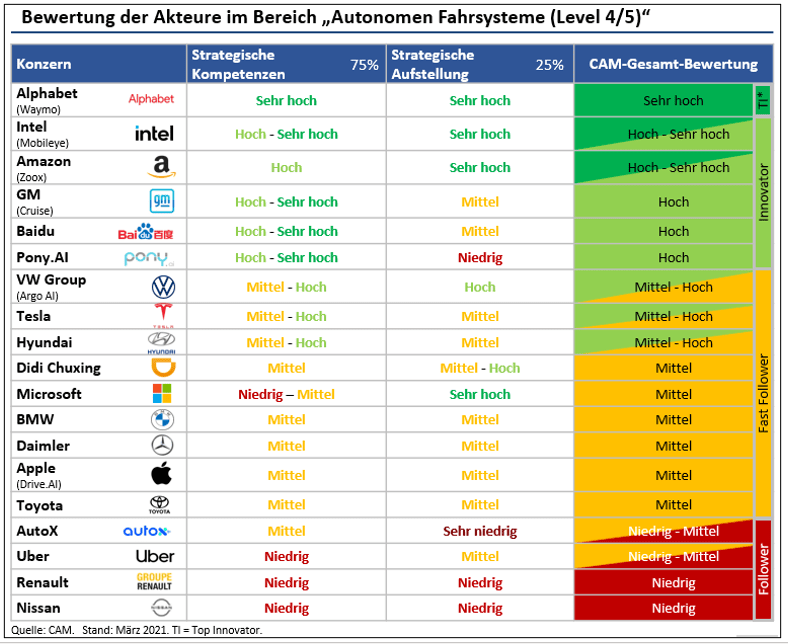
\includegraphics[width=16cm]{Figures/grafik.png}
\caption{Listas das empresas no domínio dos sistemas de condução autónoma (Nível 4/5) 2021 \cite{CAM}.}
\label{figura_companies}
\end{figure}

A partir dessa listagem, Figura \ref{figura_companies}, podemos ter uma melhor compreensão de como se encontra o cenário das empresas, na figura \textit{Konzern} em alemão, que hoje trabalham com veículos que possuem algum tipo de recurso autônomo, referente ao SAE \ref{SAE-level}. Listagem oriunda da (CAM) \textit{The Center of Automotive Management}; fornece com base em métodos científicos e bancos de dados abrangentes, orientações confiáveis sobre o universo automobilístico \cite{CAM}.

\subsubsection{VAs no mercado}

Decorrente  do aumento da automação industrial, há uma previsão do mercado mundial de veículos autônomos atingir US \$ 10 bilhões até 2024 \cite{mercadoo}. Essa previsão tem em vista o avanço da movimentação e armazenamento interno de materiais no ambiente industrial, a aplicação dos VAs nesse setor é uma tendência de mercado no interesse do investimentor \ref{implementacao}, pois os resultados gerados com a aplicação desse sistema impactam positivamente a empresa, a sociedade e a economia.

Ainda na perspectiva de crescimento econômico, e investimento no setor automobilístico em relação aos VAs. O CEO da GM, Mary Barra, diz estar investindo agressivamente no mercado de VA, com um plano de investimento de US \$35 bilhões para veículos movidos a bateria e autônomos. Tendo como expectativa arrecadar \$50 bilhões até o final da década \cite{gm}.

Além disso, espera-se que as amplicações dos VAs influenciem diferentes aspectos do sistema econômico, além do industrial, como apresenta a Figura \ref{figura_resumo}. As empresas que não conseguirem se adaptar a essas mudanças 
 de mercado terão perdas significativas. Em geral, espera-se que o valor econômico dos VAs seja bem significativo e aumente com o tempo, abrindo novas oportunidades de negócios e profissões.

\begin{figure}[H]
\centering
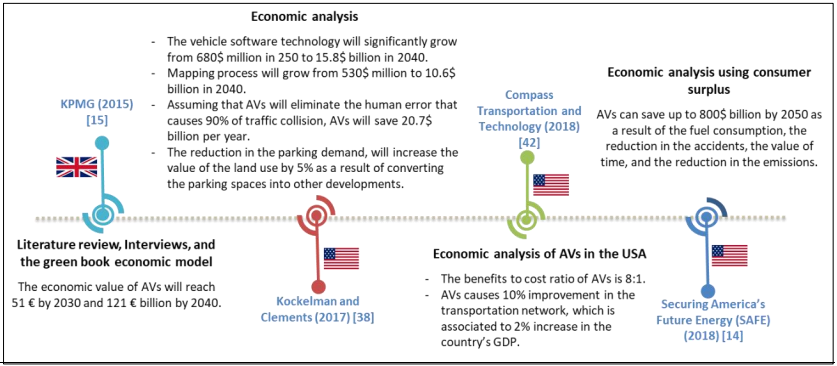
\includegraphics[width=\textwidth]{Figures/vas-mercado.png}
\caption{Resumo dos resultados de estudos anteriores que analisam o impacto dos VAs nas economias \cite{mundobrasil}.}
\label{figura_resumo}
\end{figure}

\begin{quote}
Descrição da figura \ref{figura_resumo}: apresenta um panorama econômico e do que espera-se dos veículos autonomia para as próximas décadas. Prever que os VAs terão um valor econômico de 51 bilhões de euros em 2030 e até 2040 um valor de 121 bilhões de euros. A análise, também, apresenta que devido a redução da demanda de espaço para estacionamentos o valor dessas terras irão aumentar em 5\%, pois poderão ser utilizadas em outros propósitos. Ademais, os VAs podem salvar até 800 bilhões de dólares até 2050, devido a redução do consumo de combustível e acidentes de trânsito. 
\end{quote}

Em linhas gerais, o valor econômico dos VAs vem de sua capacidade de reduzir o erro humano e melhorar a segurança no trânsito em 90\%, usos como espaço de estacionamento poderão ser utilizados para outras atividades. Pois, agora, esses veículos podem ficar circulando pela cidade ou até mesmo voltar para a residência do proprietário e voltar para buscá-lo no horário estipulado \cite{4cenarios_ocidental}. De todo modo, haverá muitas novas oportunidades de negócios criadas oriundas dos VAs \cite{mundobrasil}.




\section{Tecnologias Essenciais para a Direção Autônoma} \label{essencias_di}

Nesta seção discutiremos e apresentaremos as principais Tecnologias de Software e Hardware que fazem os VAs serem possíveis. Tudo isso, fazendo uso de Figuras e Gráficos com o intuito de facilitar o entendimento dos recursos, e de quesitos mais abstratos. 


\subsection{Como um veículo é automatizado} \label{auto}
Nesta seção cobrimos como um veículo é automatizado, seus componentes principais para se tornar um VA. Dentre as características principais de um VA, que encontramos durante nossas pesquisas, estão: a percepção, planejamento e controle.

Como representado na Figura \ref{figura_perception} um veículo necessita de 3 componentes essenciais para alcançar algum nível de automação SAE \ref{SAE-level}, sendo esses:


\begin{enumerate}
 \item \textbf{Percepção (Perception):} Busca entender o ambiente, fazendo uso de visão a partir de sensores \ref{sensores-a}, dados, localização, e redes de conexão à internet.
\item \textbf{Planejamento (Planning):} Trabalha no planejamento de ação e trajetória, guia o veículo do início ao fim, faz o planejamento de comportamento e movimento, e estipulação de tempo e da dinâmica do ambiente.
\item \textbf{Controle (Control):} Busca executar o planejamento deferido pela camada anterior, predizendo os controles para execução da tarefa designada, faz o controle dos freios, acelerador e volante, atua na geração da trajetória e controle de toda a execução.

\end{enumerate}

\begin{figure}[H]
\centering
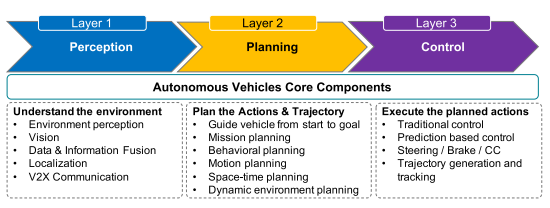
\includegraphics[width=\textwidth]{Figures/perception.png}
\caption{Componentes em camadas para obter um VA \cite{sensors-yet}.}
\label{figura_perception}
\end{figure}

As camadas representadas na figura acima (Figura \ref{figura_perception}) cada uma delas implementam diferentes operações e interagem entre si para realizar os casos de uso na direção autônoma. A Figura \ref{figura_camadas} representa essa comunicação entre camada e como essa interação acontece.

\begin{figure}[H]
\centering
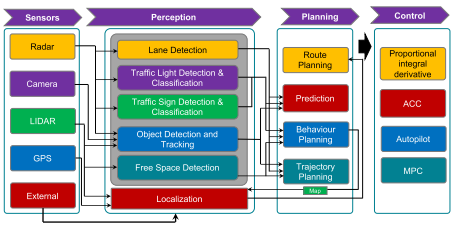
\includegraphics[width=\textwidth]{Figures/layer-sens.png}
\caption{Operações específicas de camadas e interações entre camadas \cite{sensors-yet}.}
\label{figura_camadas}
\end{figure}



\subsection{Sensores e suas funções em Veículos Autônomos} \label{sensores-a}

Como apresentado na seção anterior \ref{essencias_di}, um VA é uma categoria de veículo que pode fazer sentido do que está ao seu redor e operar sem a necessidade de intervenção humana. Desse modo, para fazer sentido do que está em sua volta é necessário recursos para essa compreensão, apresentados na Figura \ref{figura_compone}. Dentre esses recursos estão os sensores que são dispositivos que convertem eventos detectados ou mudanças no ambiente em uma medida numérica que pode então ser processada pelo componente de processamento central do veículo (visto em \ref{figura-sensores}). 
Os sensores são divididos em duas categorias com base em seu princípio operacional \cite{sensors}: 

\begin{enumerate}
 \item \textbf{Sensores de estado interno:} Conhecidos como sensores proprioceptivos, registram o estado dinâmico de um sistema dinâmico e detectam dados internos como força, taxa angular, pressão da roda, voltagem da bateria e assim por diante. Como exemplo de sensores proprioceptivos então, a unidades de medição inercial, codificadores, sensores inerciais (giroscópios e magnetômetros) e sensores de localização. 
\item \textbf{Sensores exteroceptivos:} São sensores de estado externo, por outro lado, percebem e coletam informações do ambiente do veículo, como medições de distância ou intensidade de luz de objetos. Os sensores externos incluem câmeras, detecção e alcance de rádio (Radar), detecção e alcance de luz (LiDAR) e sensores ultrassônicos (visto em \ref{figura-sensores}).

\end{enumerate}



\begin{figure}[H]
\centering
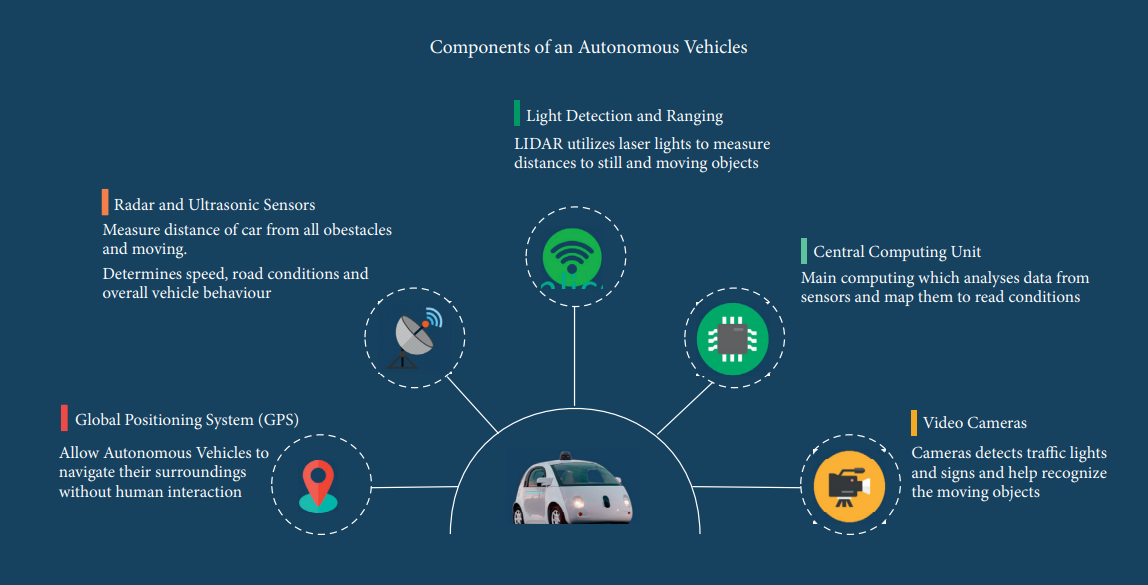
\includegraphics[width=\textwidth]{Figures/compo.png}
\caption{Componentes de um veículo autônomo \cite{aplicacao2}.}
\label{figura_compone}
\end{figure}

\begin{quote}
Descrição da Figura \ref{figura_compone}. Componentes de um VA: \textit{GPS}; permite a navegação pelo ambiente sem interação do humano. \textit{RADAR e Sensores Ultra Sônicos}; calcula a distância de obstáculos, determinada a velocidade, condição da pista e as atividades do VA no geral. \textit{LiDAR}; utiliza luz para medir a distância de objetos parados e em movimento. \textit{Computador Central}; analise os dados dos sensores e os mapeiam para entender as condições do ambiente. \textit{Câmara de Vídeo}; detecção de semáforos, sinais de trânsito e objetos em movimento.
\end{quote}

 

\subsubsection{Visão geral sobre os sensores} \label{sensores}

Esta seção é uma visão geral sobre diferentes tipos de sensores (visto na figura \ref{figura-sensores}) dos VAs com base em suas diferentes propriedades e aplicações. Examinamos, também, as vantagens e desvantagens dos três sensores básicos para percepção do ambiente utilizados do VAs na atualidade \cite{sensors}, e esses sensores são organizados como mostra a Figura \ref{figura-sensores}:


\begin{figure}[H]
\centering
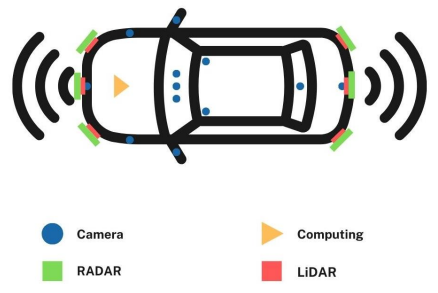
\includegraphics[width=8cm]{Figures/sensores.png}
\caption{Tipos de sensores em VAs \cite{review-auto}.}
\label{figura-sensores}
\end{figure}


A conjugação desses sensores (figura \ref{figura-sensores}) é o que possibilita os VAs. Desse modo, as figuras \ref{tabela-juncao} e \ref{all-sense} a seguir resumem essa comunicação didaticamente:

\begin{figure}[H]
\centering
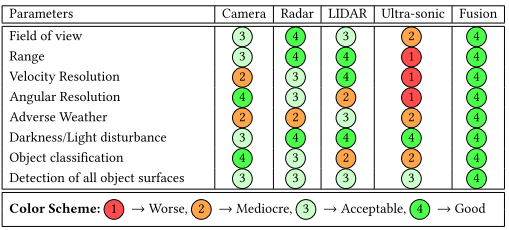
\includegraphics[width=10cm]{Figures/all-sense.png}
\caption{Adequação de sensores para diferentes situações \cite{sensors-yet}.}
\label{all-sense}
\end{figure}
\begin{quote}
Descrição da Figura \ref{all-sense}: Apresenta parâmetros para comparação entre sensores, sendo os parâmetros: \textit{Campo de visão, distância, entendimento de velocidade, resolução de ângulo, clima adverso, escuridão/distorção de luz, classificação de objetos e detecção da superfície de objetos.} Esses parâmetros são classificados de Ruim (1), Mediocre (2), Aceitável (3) e Bom (4).
\end{quote}

\begin{figure}[H]
\centering
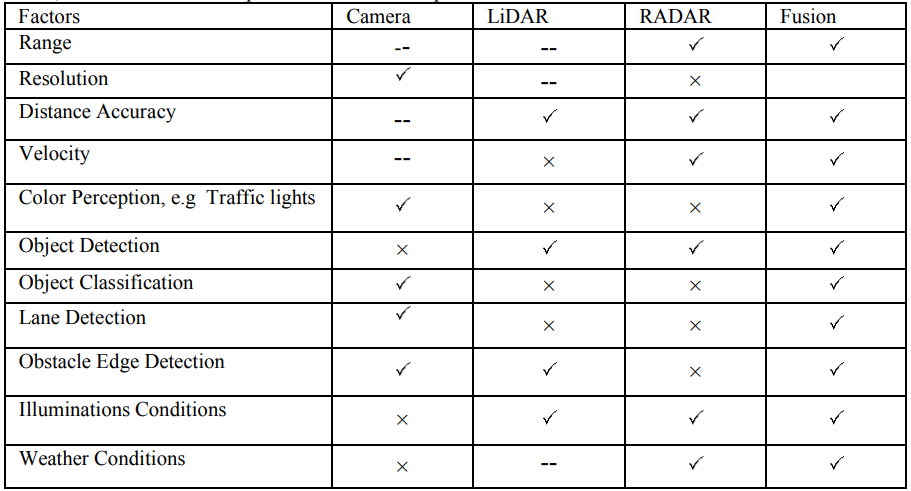
\includegraphics[width=12cm]{Figures/juncao-table.png}
\caption{Comparação comum entre sensores.}
\label{tabela-juncao}
\end{figure}
\begin{quote}
Descrição da Figura \ref{tabela-juncao}: "\checkmark" Os sensores operam completamente sob condições específicas,
"--" os sensores funcionam razoavelmente bem sob condições específicas, "x" os sensores não funcionam bem sob o fator específico em relação a outros sensores \cite{sensors}.
Os fatores analisados foram: \textit{Distância, Resolução, Precisão da distância, Velocidade, Percepção de cor, Detecção de objetos, Classificação de objetos, Detecção de faixa, Detecção de pontas de obstáculos, Condição de iluminação, Condição do ambiente}. 
\end{quote}

\subsubsubsection{Câmeras} \label{camera}

As Câmeras são uma das tecnologias mais utilizadas para observar o ambiente. Uma câmera produz imagens nítidas dos arredores detectando as luzes emitidas de uma superfície fotossensível (plano de imagem) usando uma lente de câmera (colocada na frente do sensor) \cite{sensors}. Os VAs possuem esses sensores de luz visível para fornecer uma visão de 360 graus do ambiente. As câmeras são ótimos na detecção e reconhecimento de objetos, fornecendo detalhes mais ricos e ajudando a entender os objetos sem ou com profundidade, que geralmente não são detectados por outros tipos de sensores. Dentre esses objetos estão: Sinais de trânsito (limite de velocidade, sinais de parada, sinais de ultrapassagem), semáforos, pedestres, animais são alguns exemplos de tais objetos sem ou com profundidade \cite{sensors-yet}. Esses dados coletados com as câmeras são enviados para os algoritmos baseados em IA para uso posterior, e criação de uma imagem 2D \cite{aplicacao2}. 
No entanto, esses sensores são imprecisos em ambientes escuros e geram uma grande quantidade de dados para processar. Outros tipos de câmeras como as infravermelhas, também, são utilizadas para melhor desempenho em condições de baixa visibilidade \cite{review-auto}. As câmeras são dispostas nos VAs como mostrado na Figura \ref{figura-sensores}, e para detalhes específicos dos diferentes modelos de câmeras e suas características apresentamos na Figura \ref{tabela-camera}.

\begin{figure}[H]
\centering
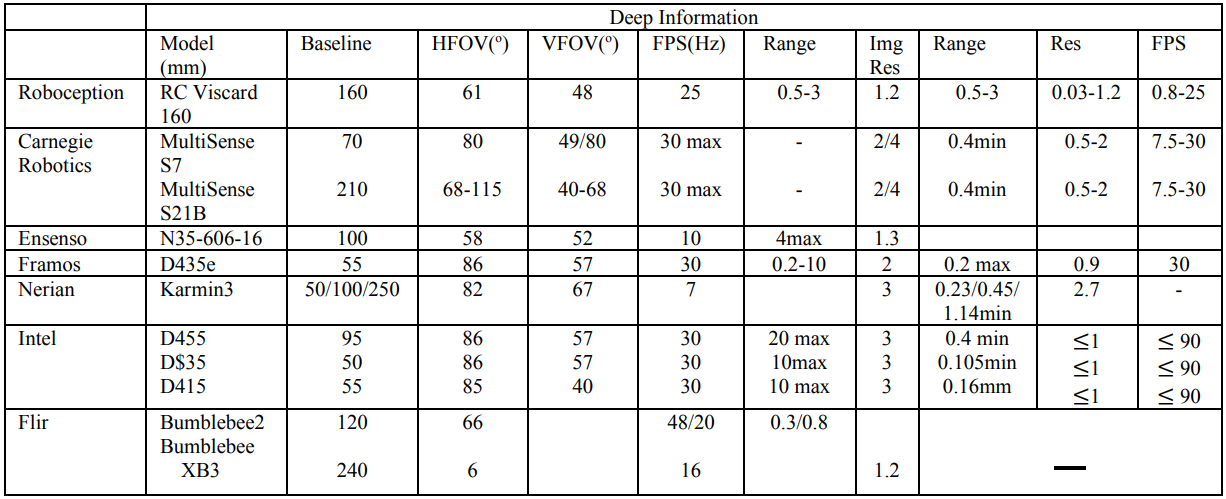
\includegraphics[width=\textwidth]{Figures/camera-table.png}
\caption{Especificações gerais da câmera estéreo.}
\label{tabela-camera}
\end{figure}
\begin{quote}
Descrição da Figura \ref{tabela-camera}: Campo de visão horizontal (HFOV), Campo de visão vertical (VFOV), Quadros por segundo (FPS), Resolução da imagem em megapixels (Res Img), Quadros de profundidade por segundo (FPS) \cite{sensors}.
\end{quote}
\subsubsubsection{LiDAR}

O LiDAR, ou detecção e alcance de luz, foi desenvolvido pela primeira vez na década de 1960 e desde então tem sido amplamente empregado no mapeamento de terreno aeronáutico e aeroespacial \cite{sensors}. Nos VAs os LiDAR são sensores que usa a luz como meio para medir distâncias é calculado medindo o tempo que a luz leva para ser refletida no receptor, e são dispostos no VA como mostrado na Figura \ref{figura-sensores}. Tais sistemas emitem feixes de laser que atingem o ambiente e refletem para um fotodetector. Os feixes coletados em tempo real e de maneira confiável, e  são convergidos juntos como uma nuvem de pontos criando uma imagem 3D do ambiente \cite{aplicacao2}. Dado que os LIDARs são sensores sem profundidade, eles não são capazes de identificar os elementos sem profundidade, como semáforos, sinais de trânsito e assim por diante.
Embora o LiDAR seja um sensor poderoso e eficiente para o uso em VAs, acabam por ser  bastante caros e aumentando o valor final do VA \cite{review-auto}. 
Os LiDAR em VAs são dispostas como mostrado na Figura \ref{figura-sensores}, e para mais detalhes específicos e diferentes características do LiDAR, verificar a seguinte Figura \ref{tabela-lidar}.

\begin{figure}[H]
\centering
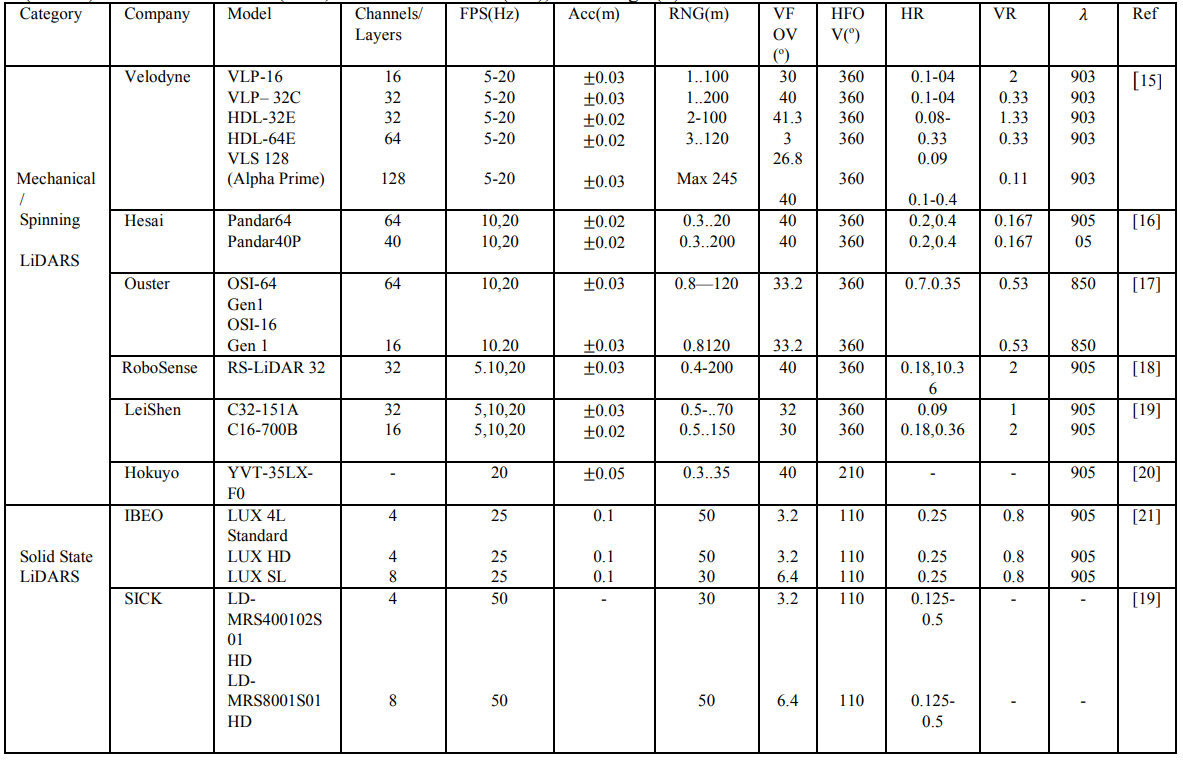
\includegraphics[width=\textwidth]{Figures/lidar-table.png}
\caption{Especificações gerais de LiDAR.}
\label{tabela-lidar}
\end{figure}

\begin{quote}
Descrição da Figura \ref{tabela-lidar}: Quadro por segundo (FPS), Precisão (Acc), Alcance de detecção (RNG), FoV vertical (VFOV), FoV horizontal (HFOV) Resolução horizontal (HR0, Resolução vertical (VR), Comprimento de onda ($\lambda$) \cite{sensors}.
\end{quote}


\subsubsubsection{Radares}



Antes da Segunda Guerra Mundial, foi desenvolvido o \textit{Radio Detection and Ranging}, ou Radar. Cujo tem como essência emitir ondas eletromagnéticas dentro da região de interesse e receber ondas dispersas (ou reflexões) de alvos para processamento de sinal e determinação a informações que alcançam \cite{sensors}. Trabalhando com essas ondas de rádio para calcular fatores como a distância, velocidade e ângulo. Com a ajuda desses transmissores de radar, os VAs podem emitir ondas de rádio e receber as ondas refletidas com a ajuda de receptores de radar. O radar funciona bem na maioria dos climas e em longas distâncias, mas pode identificar objetos falsamente \cite{review-auto}.
Os Radares em VAs são dispostas como mostrado na Figura \ref{figura-sensores}, e para mais detalhes específicos e diferentes características dos Radares, verificar a seguinte Figura \ref{tabela-radar}.



\begin{figure}[H]
\centering
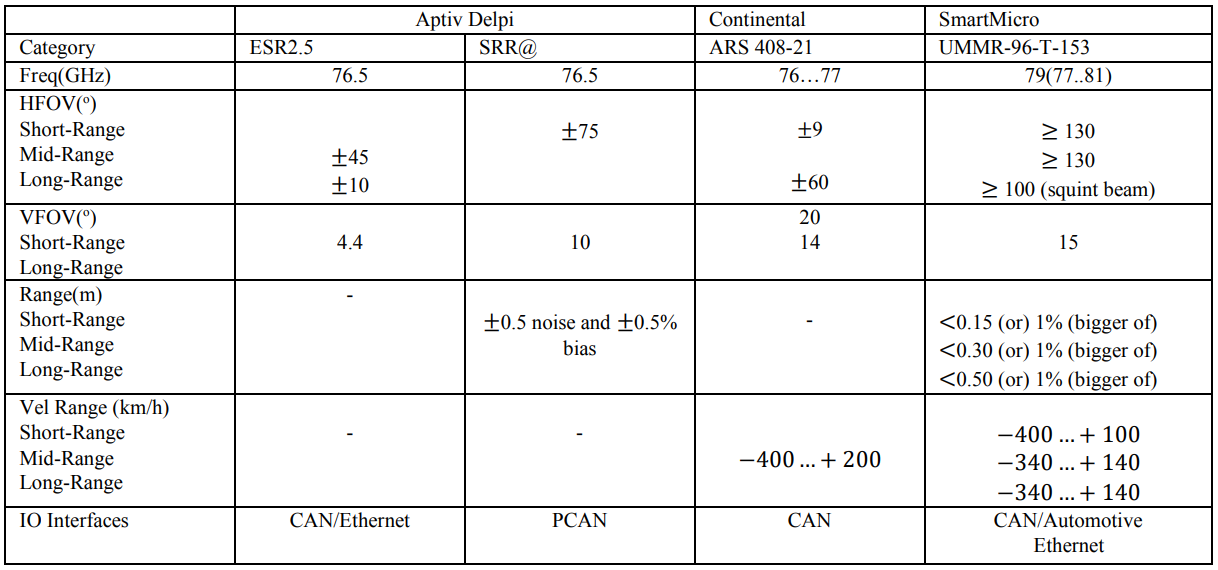
\includegraphics[width=\textwidth]{Figures/radar-table.png}
\caption{Especificação geral de sensores RADAR.}
\label{tabela-radar}
\end{figure}

\begin{quote}

Descrição da Figura \ref{tabela-radar}:  Acrônimos primeiro da primeira coluna de cima para baixo, Frequência (Freq), FoV horizontal (HFOV), FoV vertical (VFOV), Precisão de alcance (Faixa Acc), Faixa de velocidade (Faixa Vel), ROS (Sistema operacional robótico) \cite{sensors}.
\end{quote}


\subsubsection{Sistemas avançados de assistência ao condutor} \label{adas}


Como apresentado em seções anteriores \ref{nv3} e \ref{SAE-level}, os VAs possuem tecnologias de assistência ao condutor ou ADAS visando aumentar a segurança e conforto dos VAs. Essas tecnologias de assistência ao motorista são comumente empregadas nos VAs de nível 1 a 3 SAE \ref{SAE-level}.

\subsubsubsection{Controle de Cruzeiro} \label{cruzeiroo}

O Controlador de Cruzeiro foi introduzido pela primeira vez no mercado automotivo na década de 1980, o controle de cruzeiro apareceu no início do século XX, operado por um dispositivo chamado governador centrífugo que regulava a velocidade com base na quantidade de combustível injetado \cite{caio}. Essa funcionalidade, na atualidade, é capaz de ajustar automaticamente a velocidade do veículo mantendo uma distância constante do veículo seguinte e é conhecida comumente como controle de cruzeiro \cite{sensors-yet}.
A partir disso os VAs são capazes de evitar possíveis colisões, emitindo sinais sonoros para o condutor, e reduzindo a velocidade do veículo até alcançar uma distância segura. Hoje, esse sistema é conhecido como controle de cruzeiro adaptativo ou \textit{Adaptive Cruise Control} (ACC) baseado em radares e câmeras que medem a distância, velocidade e ângulo de aproximação entre os veículos nas estradas como ilustrado nas Figuras \ref{cruzeiro} e \ref{ACC}:

\begin{figure}[H]
\centering
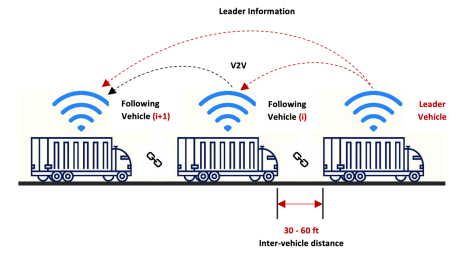
\includegraphics[width=10cm]{Figures/cruzeiro.png}
\caption{Distância entre veículos \cite{review-auto}.}
\label{cruzeiro}
\end{figure}


\begin{figure}[H]
\centering
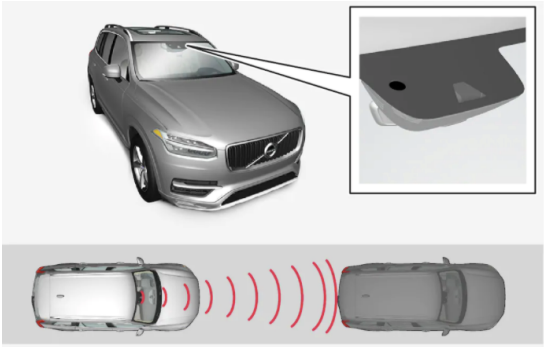
\includegraphics[width=10cm]{Figures/ACC.png}
\caption{Controle de Cruzeiro adaptativo em um carro da Volvo \cite{caio}.}
\label{ACC}
\end{figure}


\subsubsubsection{Assistente de permanência na faixa} \label{faixa}

Assistente de Permanência na Faixa auxilia o motorista a manter o veículo na faixa e emite avisos quando o veículo sai da faixa. Também é muito útil para avisar os motoristas quando eles estão cansados e sonolentos \cite{caio}. A seguir a Figura \ref{assistente} apresenta o funcionamento do assistente:

\begin{figure}[H]
\centering
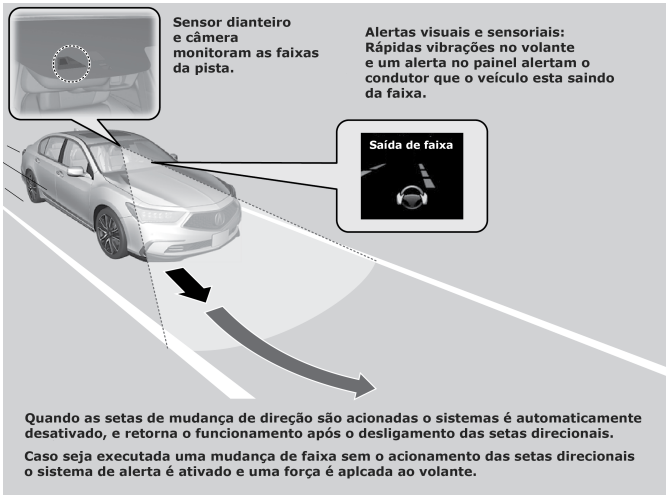
\includegraphics[width=\textwidth]{Figures/assistente.png}
\caption{Funcionamento do assistente de permanência de faixa \cite{caio}.}
\label{assistente}
\end{figure}

\subsubsubsection{Assistente de estacionamento} \label{estacionamento}


Um sistema de assistência ao estacionamento, também conhecido por Park Assist, tem como objetivo realizar as manobras de estacionamento de forma autónoma. Por meio de sensores (Figura \ref{figura-sensores}) ao redor do veículo, o sistema calcula o tamanho do espaço para manobra (Figura \ref{cruzeiro}) e faz o movimento necessário para estacionar o veículo com total segurança. Nesse cenário, o veículo assume o controle da direção e dos pedais, evitando qualquer obstáculo, contudo o motorista presente deve estar sempre atento a qualquer imprevisto ou solicitação do veículo \cite{caio}. Essa função é presente nos VAs de nível 2 SAE, como apresendado na seção \ref{nv3} 

\subsection{Arquiteturas e Algoritmos} \label{arq_alg}

Nesta subseção apresentaremos os Software, Algoritmos e Arquiteturas que possibilitam os VAs interpretarem o ambiente a sua volta, e tomarem decisões com base nesses dados. 


\subsubsection{Inteligência artificial} \label{ia}

Ao longo da história, os seres humanos tiveram que aprender e realizar tarefas que dependiam do seus próprios conhecimentos e inteligência para serem executadas, desde empilhar gravetos até cálculos matemáticos, programação de software, e no nosso caso condução de um veículo. Diante disso, muito esforço tem sido feito nas últimas décadas para desenvolver vários sistemas de computação capazes de substituir humanos nessas tarefas, e muitas dessas pesquisas para construir esses tipos de sistemas podem ser atribuídas ao campo da inteligência artificial (IA) \cite{caio}. 
Existem muitas definições para IA e seus subcampos, muitas das quais baseadas nas capacidades e comportamentos de um agente sob uma visão de domínio, o que significa que um agente pode ser definido operacionalmente em termos do ambiente em que atua.
Um agente, para o cenário de um VA, deve ter a seguinte característica principal: a autonomia, o que significa que deve tomar a iniciativa e exercer controle sobre suas ações, e conduzir negociações com agentes humanos ou outros VAs de modo a continuar com o seu DDT.
Essa característica é com base em estratégias de argumentação, o agente, portanto, pode tomar decisões e tirar conclusões. 

Em geral, a inteligência artificial refere-se à capacidade de um computador ou máquina de imitar as habilidades da mente humana \cite{software-ia} como percepção visual, reconhecimento de fala, tomada de decisão e processamento de linguagem natural. O campo da IA envolve a criação de algoritmos, modelos e software que podem aprender e se adaptar a novos dados e situações, permitindo que as máquinas executem tarefas que, de outra forma, exigiriam intervenção humana. Tendo muitas aplicações diferentes, incluindo aprendizado de máquina (apresentado em \ref{machine}) e aprendizagem profunda (apresentado em \ref{Profunda}), visão computacional, processamento de linguagem natural, robótica, entre outros, apresentados nesse relatório, que fazem parte de um VA. O aprendizado de máquina e aprendizagem profunda, em particular, são um subconjuntos da IA que envolve algoritmos de treinamento para reconhecer padrões nos dados e fazer previsões ou decisões com base nesses dados. Esse processo é frequentemente usado em campos como análise de dados, análise fincanceira, veículos autônomos, segurança cibernética, etc \cite{software-review, software-cnn}.


\subsubsubsection{Aprendizado de Máquina} \label{machine}

O aprendizado de máquina é um subcampo da inteligência artificial \ref{ia} que se concentra no desenvolvimento de algoritmos e modelos estatísticos que permitem que os sistemas de computador aprendam automaticamente com os dados e melhorem seu desempenho em uma determinada tarefa sem serem explicitamente programados. Em outras palavras, envolve o treinamento de programas de computador para reconhecer padrões e relacionamentos nos dados e, em seguida, usar esse conhecimento para fazer previsões ou decisões. Os algoritmos de aprendizado de máquina podem ser usados em uma ampla variedade de aplicativos, como reconhecimento de imagem \cite{review-auto} e fala, processamento de linguagem natural, detecção de fraude, sistemas de recomendação e análise preditiva. Alguns tipos comuns de aprendizado de máquina incluem aprendizado supervisionado, aprendizado não supervisionado e aprendizado por reforço. \cite{software-review, software-cnn}.

Diante disso, podemos identificar que o Aprendizado de Máquina está presente em muitas atividades diárias da vida humana, por ex:. ao projetar a forma como uma rede social é apresentada a cada usuário, que tipo de anúncios e matérias são exibidos dependendo das preferências e consultas de pesquisa do usuário, separando e-mail confiável de spam e até câmeras de celular e teclado. Tudo isso, fazendo uso de algoritmos para coletar dados, permitindo que os computadores resolvam problemas e tomem decisões com base em seu próprio conhecimento adquirido ao longo do tempo \cite{caio}. Desse modo, nos VAs o aprendizado de máquina pode ser usado para funções como o ADAS, apresentado em \ref{adas}, para aprimorar todo o desempenho de um veículo. O ML desempenha diversas funções na operação rotineira de um VA, como: classificação de objetivos, controle dos pedais, faróis, sistemas de assistências \ref{adas} \cite{aplicacao2}.

\subsubsubsection{Aprendizagem Profunda} \label{Profunda}

O Aprendizado Profundo é um subconjunto do aprendizado de máquina que envolve o treinamento de redes neurais artificiais para aprender com grandes quantidades de dados. O termo "profundo" refere-se às múltiplas camadas que compõem essas redes neurais, que são projetadas para imitar a estrutura do cérebro humano. No aprendizado profundo, a rede neural é treinada em um grande conjunto de dados usando um algoritmo que ajusta os pesos da rede para minimizar a diferença entre a saída da rede e a saída desejada. Esse processo é repetido várias vezes até que a rede seja capaz de classificar ou prever com precisão novos dados que nunca viu antes \cite{software-cnn}. O aprendizado profundo revolucionou muitos campos, incluindo visão computacional, processamento de linguagem natural e reconhecimento de fala, entre outros \cite{review-auto, software-review}. 

Sendo o Deep Learning (DL) ou Aprendizado Profundo uma das ferramentas mais eficazes no campo do Aprendizado de Máquina. Como apresentado, o DL insere dados de maneira hierárquica, incorporando propriedades globais e imutáveis cada vez mais abstratas em cada nível de processamento. O DL aprende as características de um conjunto de dados e as combina para atingir um objetivo específico.

Essas múltiplas camadas no DL para perceptiva de um VA são: camada de entrada, uma camada oculta e uma camada de saída. Listadas \cite{software-ia}:

\begin{enumerate}
 \item \textbf{A camada de entrada:} A camada de entrada para DL trata uma grande quantidade de dados adquiridos de várias fontes. O grande conjunto de dados para modelagem de trânsito é diversificado e vem de várias fontes, como câmeras, LIDAR, sensores, sendo dados quase em tempo real fornecidos pelo equipamento colocado nos VAs \ref{figura-sensores}.
\item \textbf{A camada oculta:} A camada oculta é responsável por processar os dados de entrada, extraindo informações úteis para criar novos atributos que são usados como entrada para o modelo DL. Cada camada dentro da camada oculta recebe regras que se concentram nos atributos de dados de entrada que são atualizados de acordo com a nova entrada de dados. O tamanho da camada oculta é expresso pelo número de neurônios ali presentes. Os neurônios têm uma influência importante na capacidade de aprendizado do algoritmo; muito poucos podem levar ao sub aprendizado e muitos podem levar à super adaptação. Esse número  de camadas varia de aplicação para aplicação.
\item \textbf{A camada de Saída:} A camada de saída é responsável por exportar os valores ou vetores de valores que estejam de acordo com o formato exigido pelo problema e apresentar os resultados visuais com base nas medições estatísticas de erros.
\end{enumerate}

\subsubsection{Redes Neurais Artificiais aplicadas a Veículos Autônomos}

As Redes Neurais Artificiais (RNAs) têm sido amplamente aplicadas no desenvolvimento de VAs devido à sua capacidade de processar grandes quantidades de dados, aprender com exemplos e fazer previsões. As RNAs podem ser usadas para uma variedade de tarefas em VAs, incluindo percepção, tomada de decisão e controle \cite{sensors-yet}. 

Como visto, a percepção é um dos componentes mais críticos dos VAs \ref{auto}, e as RNAs têm sido usadas para melhorar a precisão da percepção de várias maneiras. 
Por exemplo, as  RNAs têm sido usadas para detectar e classificar objetos de dados oriundos de sensores (vistos em \ref{sensores}) , como: LiDER, câmeras e RADAR, que podem ser usadas para criar mapas precisos do ambiente em volta do veículo. 
As RNAs também, como apresentado nas subseções \ref{cruzeiroo} e \ref{camera}, podem ser usadas para identificar e rastrear outros veículos, pedestres e obstáculos, o que é crítico para uma operação segura e confiável de um VA.

O planejamento de decisão é outro componente crítico dos VAs, e as  RNAs têm sido usadas para tomar decisões com base em dados de sensores e informações ambientais. Por exemplo, as RNAs podem ser treinadas para prever o comportamento de outros usuários da estrada, como outros veículos, pedestres e ciclistas, e usar essas informações para tomar decisões como quando mudar de faixa ou diminuir a velocidade \cite{aplicacao2}. As RNAs também podem ser usadas para determinar a melhor rota a seguir com base no tráfego e nas condições da estrada. 

O controle é o componente final dos VAs, e as RNAs têm sido usadas para controlar os movimentos do veículo. Por exemplo, as  RNAs podem ser usadas para controlar a direção, aceleração e frenagem do veículo, que podem ser usadas para manter o veículo em sua faixa, manter uma distância segura de outros veículos e evitar colisões, visto em \ref{cruzeiroo}, \ref{faixa} e \ref{estacionamento}.

No geral, as RNAs têm sido uma tecnologia crucial no desenvolvimento de VAs. À medida que continuam a melhorar, elas provavelmente desempenharam um papel cada vez mais importante no desenvolvimento dos VAs, tornando-os mais seguros, eficientes e confiáveis \cite{sensors-yet, aplicacao2}.


Entretanto, a constante variação de imagem em ambientes relacionados à visibilidade do veículo levanta algumas questões relacionadas aos VAs e a sua capacidade de identificar e  entender o ambiente à sua volta, considerando que as tecnologias de processamento de imagem e reconhecimento de padrões podem falhar mesmo que funcionem bem em algumas situações. Esse problema pode ser demonstrado justamente porque essas tecnologias podem não se adaptam bem a diferentes ambientes \cite{caio}. Diante disso, é necessário o uso de diferentes algoritmos e sensores (apresentados em \ref{sensores}) para que os componentes (visto em \ref{figura_perception}) do VA sejam capazes de fazer total sentido do ambiente de ação.

Desse modo, nessas seções \ref{cnn}, \ref{r-cnn}, \ref{rnn} e \ref{LSTM-s} iremos tratar dos principais algoritmos encontrados aplicados aos VAs e seus objetivos na identificação de imagens, processamentos, e classificações.

\subsubsubsection{Redes Neurais Convolucionais} \label{cnn}

No caminho de processar e compreender os dados coletados pelos sensores dos VAs, temos as Redes Neurais Convolucionais em inglês, \textit{Convolutional Neural Networks} (CNN). Esse tipo de rede neural é utilizada para processamento de imagens por apresentar alta precisão na extração de características distintivas de imagens utilizando a função de convolução. É preciso entrada 2D e usar várias camadas ocultas para extrair recursos de alto nível. Depois de receber a entrada, ele identifica padrões úteis nas imagens com base na organização espacial dos pixels de entrada. Como nenhum pré-processamento é necessário, a CNN pode ser facilmente implantada. Em VAs, eles são usados para planejamento de caminhos e detecção de pedestres \cite{review-auto}.

\begin{figure}[H]
\centering
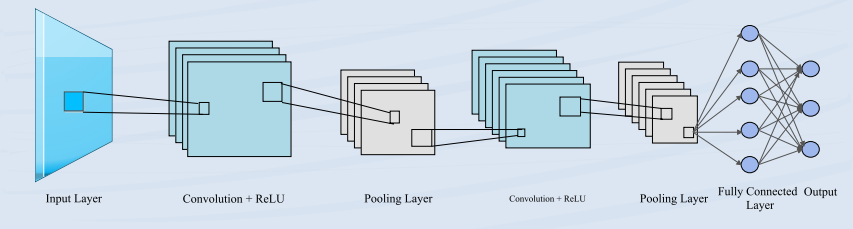
\includegraphics[width=\textwidth]{Figures/CNN.png}
\caption{Estrutura da CNN \cite{software-cnn}.}
\label{CNN}
\end{figure}

As \textit{Redes Neurais Convolucionais} (Figura \ref{CNN}) incluem camadas de convolução, onde um filtro com pesos que podem ser aprendidos é convoluído sobre a entrada, camadas de agrupamento, que reduzem o tamanho espacial da entrada por subamostragem e camadas totalmente conectadas, que mapeiam sua entrada para dimensão de saída desejada. Como apresentado, as CNNs são comumente usadas para extrair recursos de dados de imagem, alcançando resultados bem-sucedidos no domínio da visão computacional \cite{software-review}.

\subsubsubsection{R-CNN, fast R-CNN, faster R-CNN} \label{r-cnn}

Ao detectar o objeto em uma imagem com CNN convencional \ref{CNN}, o tamanho da camada de saída varia porque o número de ocorrências do objeto não é estático, fazendo a requisição de técnicas mais complexas para resolver em comparação com a classificação de imagens. \cite{software-cnn}.
Por conta disso, quando tratamos sobre identificação de objetos em imagens, temos o \textit{Region Convolution Neural Network} (R-CNN) que usa um processo de pesquisa seletiva para identificar os limites e rótulos de cada objeto em uma imagem e criar uma caixa de limite ao redor deles. A caixa delimitadora é finalmente submetida a um modelo de regressão linear para encontrar coordenadas precisas para a caixa. Nos VAs, o RCNN é usado para detecção de pedestres, objetos e sinais de trânsito \cite{review-auto}.


\subsubsubsection{Rede Neural Recorrente} \label{rnn}

As Rede Neural Recorrente no inglês \textit{Recurrent Neural Networks} (RNN) são algoritmos que trabalham bem com dados sequenciais e de séries temporais, e lida bem com problemas espaço-temporais. A rede neural recorrente mais simples pode ser considerada como uma extensão da rede neural totalmente conectada de duas camadas, onde a camada oculta tem um feedback. Esta pequena alteração permite modelar dados sequenciais de forma mais eficiente. A cada etapa da sequência, a RNN processa os dados de entrada da etapa atual juntamente com a memória das etapas anteriores, que é transportada nos neurônios ocultos anteriores, como ilustrado na Figura \ref{RNN}.

\begin{figure}[H]
\centering
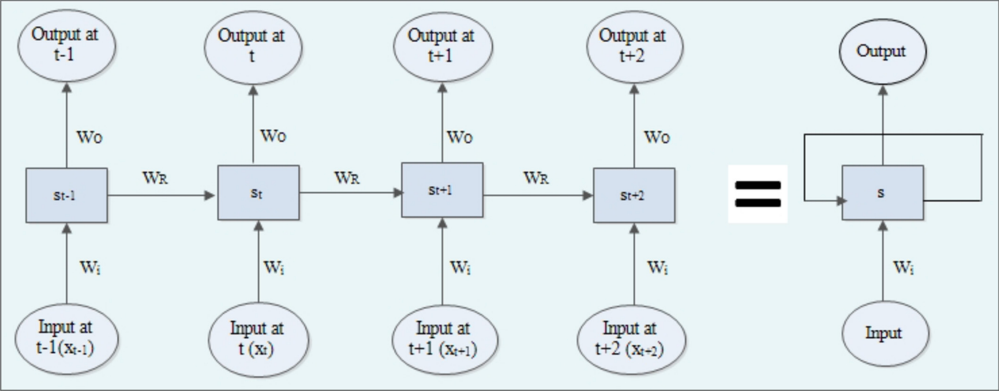
\includegraphics[width=\textwidth]{Figures/RNN.png}
\caption{Estrutura de uma RNN \cite{software-cnn}.}
\label{RNN}
\end{figure}

No entanto, RNN não pode ser usado para prever a próxima palavra em uma sequência, para detectar o comportamento dos motoristas com base no histórico anterior, prever o consumo de energia de uma casa, etc \cite{software-cnn}. Ademais, é difícil treinar essa rede para aprender sequências longas na prática devido ao desaparecimento ou explosão do gradiente, razão pela qual RNNs com “portas” são introduzidas. Em cada célula dessas redes, em vez de uma simples camada oculta totalmente conectada, uma arquitetura fechada é implantada. 

As três variantes mais comuns de RNNs são memória de longo prazo no inglês \textit{Long Short term Memory} (LSTM), \textit{Time Delay Neural Network} (TDNN) e \textit{Gated Recurrent Unit} (GRU), que são discutidas a seguir.
A LSTM e a unidade recorrente Gated (GRU) são as RNNs fechadas mais comumente usadas, e na previsão do comportamento de veículos, e os LSTMs são os modelos profundos mais usados \cite{software-review}.


\subsubsubsection{Redes de Memória de Longo Curto Prazo} \label{LSTM-s}

Nas RNNs convencionais \ref{rnn}, o efeito da entrada passada decai exponencialmente na saída à medida que percorre a conexão recorrente. Para solucionar essa perda de "memória" das informações já processadas as LSTMs são introduzidas, sendo consideradas melhores do que o RNN devido às suas características de lembrar seletivamente de padrões por um longo período de tempo, lidando com dados de séries temporais tanto para longa e curta duração \cite{software-cnn}.

\begin{figure}[H]
\centering
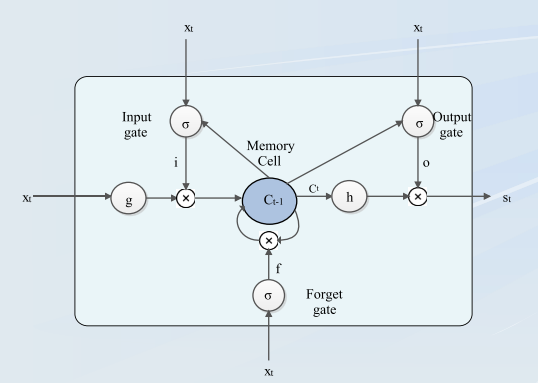
\includegraphics[width=\textwidth]{Figures/LSTM.png}
\caption{Estrutura de uma LSTM \cite{software-cnn}.}
\label{LSTM}
\end{figure}



Para prever a intenção dos veículos, um LSTM é usado como um classificador de sequência. Nesta tarefa, uma sequência de características são alimentadas a células sucessivas de um LSTM. Em seguida, o estado oculto da última célula na sequência é mapeado para a dimensão de saída, a entrada é incorporada usando uma camada totalmente conectada e alimentada a uma camada de três camadas \cite{software-review}, como representado na Figura \ref{LSTM}.




\chapter{Conclusões} \label{concl}

O \textit{objetivo} \ref{Objetivos} desse primeiro ano de pesquisa foi realizar um estudo da bibliografia existente para entender e mapear as perspectivas e tecnologias dos Veículos Autônomos, fazendo o paralelo do Brasil com o que há de melhor da área no mundo. 

Desse modo, foi possível identificar as perspectivas sobre implementação dos veículos autônomos (VAs), assim como os seus benefícios, e suas desvantagens, áreas de aplicação, e os países mais adequados para sua aplicação, e suas tendências de mercado para o Brasil e o mundo.
Ademais, apresentamos e estruturamos os diferentes níveis de condução autonomia, entendemos e apresentamos quais objetivos econômicos e tecnológicos as principais empresas pelo mundo tem com essa tecnologia.
Além do mais, mapeamos as tecnologias essenciais para o funcionamento de um VA, e a partir dos levantamentos bibliográficos foi possível apresentar de maneira didática os principais Software e Hardware que fazem dessa tecnologia possível.
Ao fazer isso, realizamos todos os \textit{Objetivos} \ref{Objetivos} propostos no \textit{Plano de Trabalho}.

Todavia, esse projeto buscou trazer um aprendizado dos conhecimentos teóricos sobre os VAs, visando um segundo ano de projeto onde será possível fazer a  aplicação dos softwares apresentados neste relatório.

Portanto, apesar do sucesso em mapear as perspectivas e tecnologias dos VAs, precisamos colocar esses conhecimentos relacionados à parte de softwares em prática.



\chapter{Perspectiva de continuidade} \label{continuidade}

De acordo com os \textit{objetivos} \ref{Objetivos} propostos no projeto deste ano, nos propomos a um segundo ano visando colocar em prática os conhecimentos aqui obtidos e dar continuidade e aprofundamento no âmbito de Software para VAs. Visto que, neste ano, fizemos o levantamento bibliográfico, mapeamento e compreensão das \textit{Tecnologias Essenciais para a Direção Autônoma} \ref{essencias_di} e mais especificamente das \textit{Arquiteturas e Algoritmos} \ref{arq_alg} cujo será o foco da continuidade. Portanto, temos a perspectiva de fazermos a seleção e a testagem dos Algoritmos de Controle de VAs relevantes para a continuidade do projeto.

\chapter{Participação em congressos e trabalhos publicados ou submetidos e outras
atividades acadêmicas e de pesquisa} \label{eventos}

Também apresentamos os certificados dos minicursos oferecidos pela plataforma Instituto de Tecnologia e Sociedade e Coursera  nas figuras \ref{Google} \ref{Design} e \ref{Direitos}.


\begin{figure}[H]
\centering
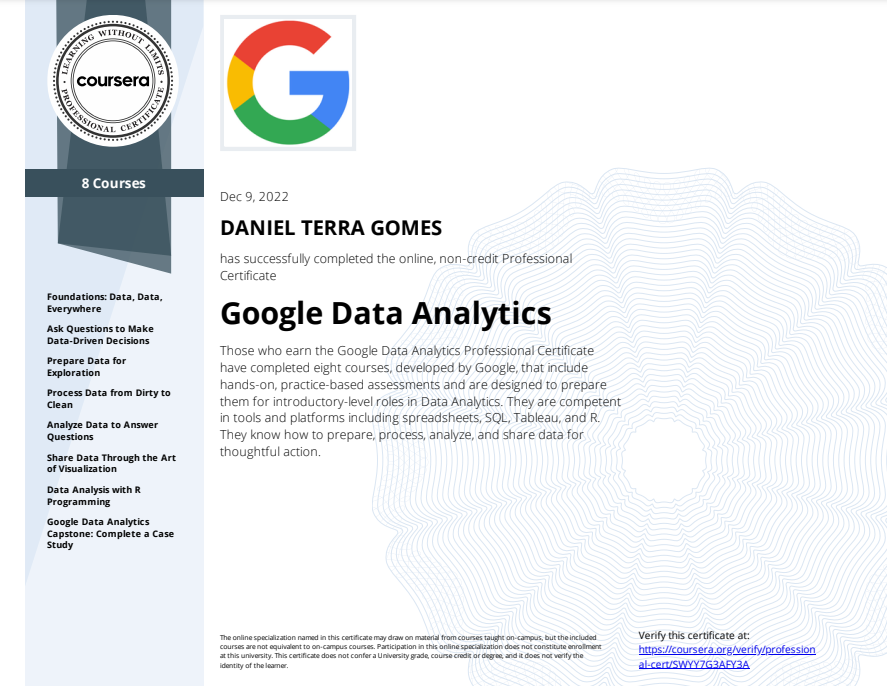
\includegraphics[width=\textwidth]{Figures/google.png}
\caption{Certificado de conclusão do curso Google Data Analytics.}
\label{Google}
\end{figure}

\begin{figure}[H]
\centering
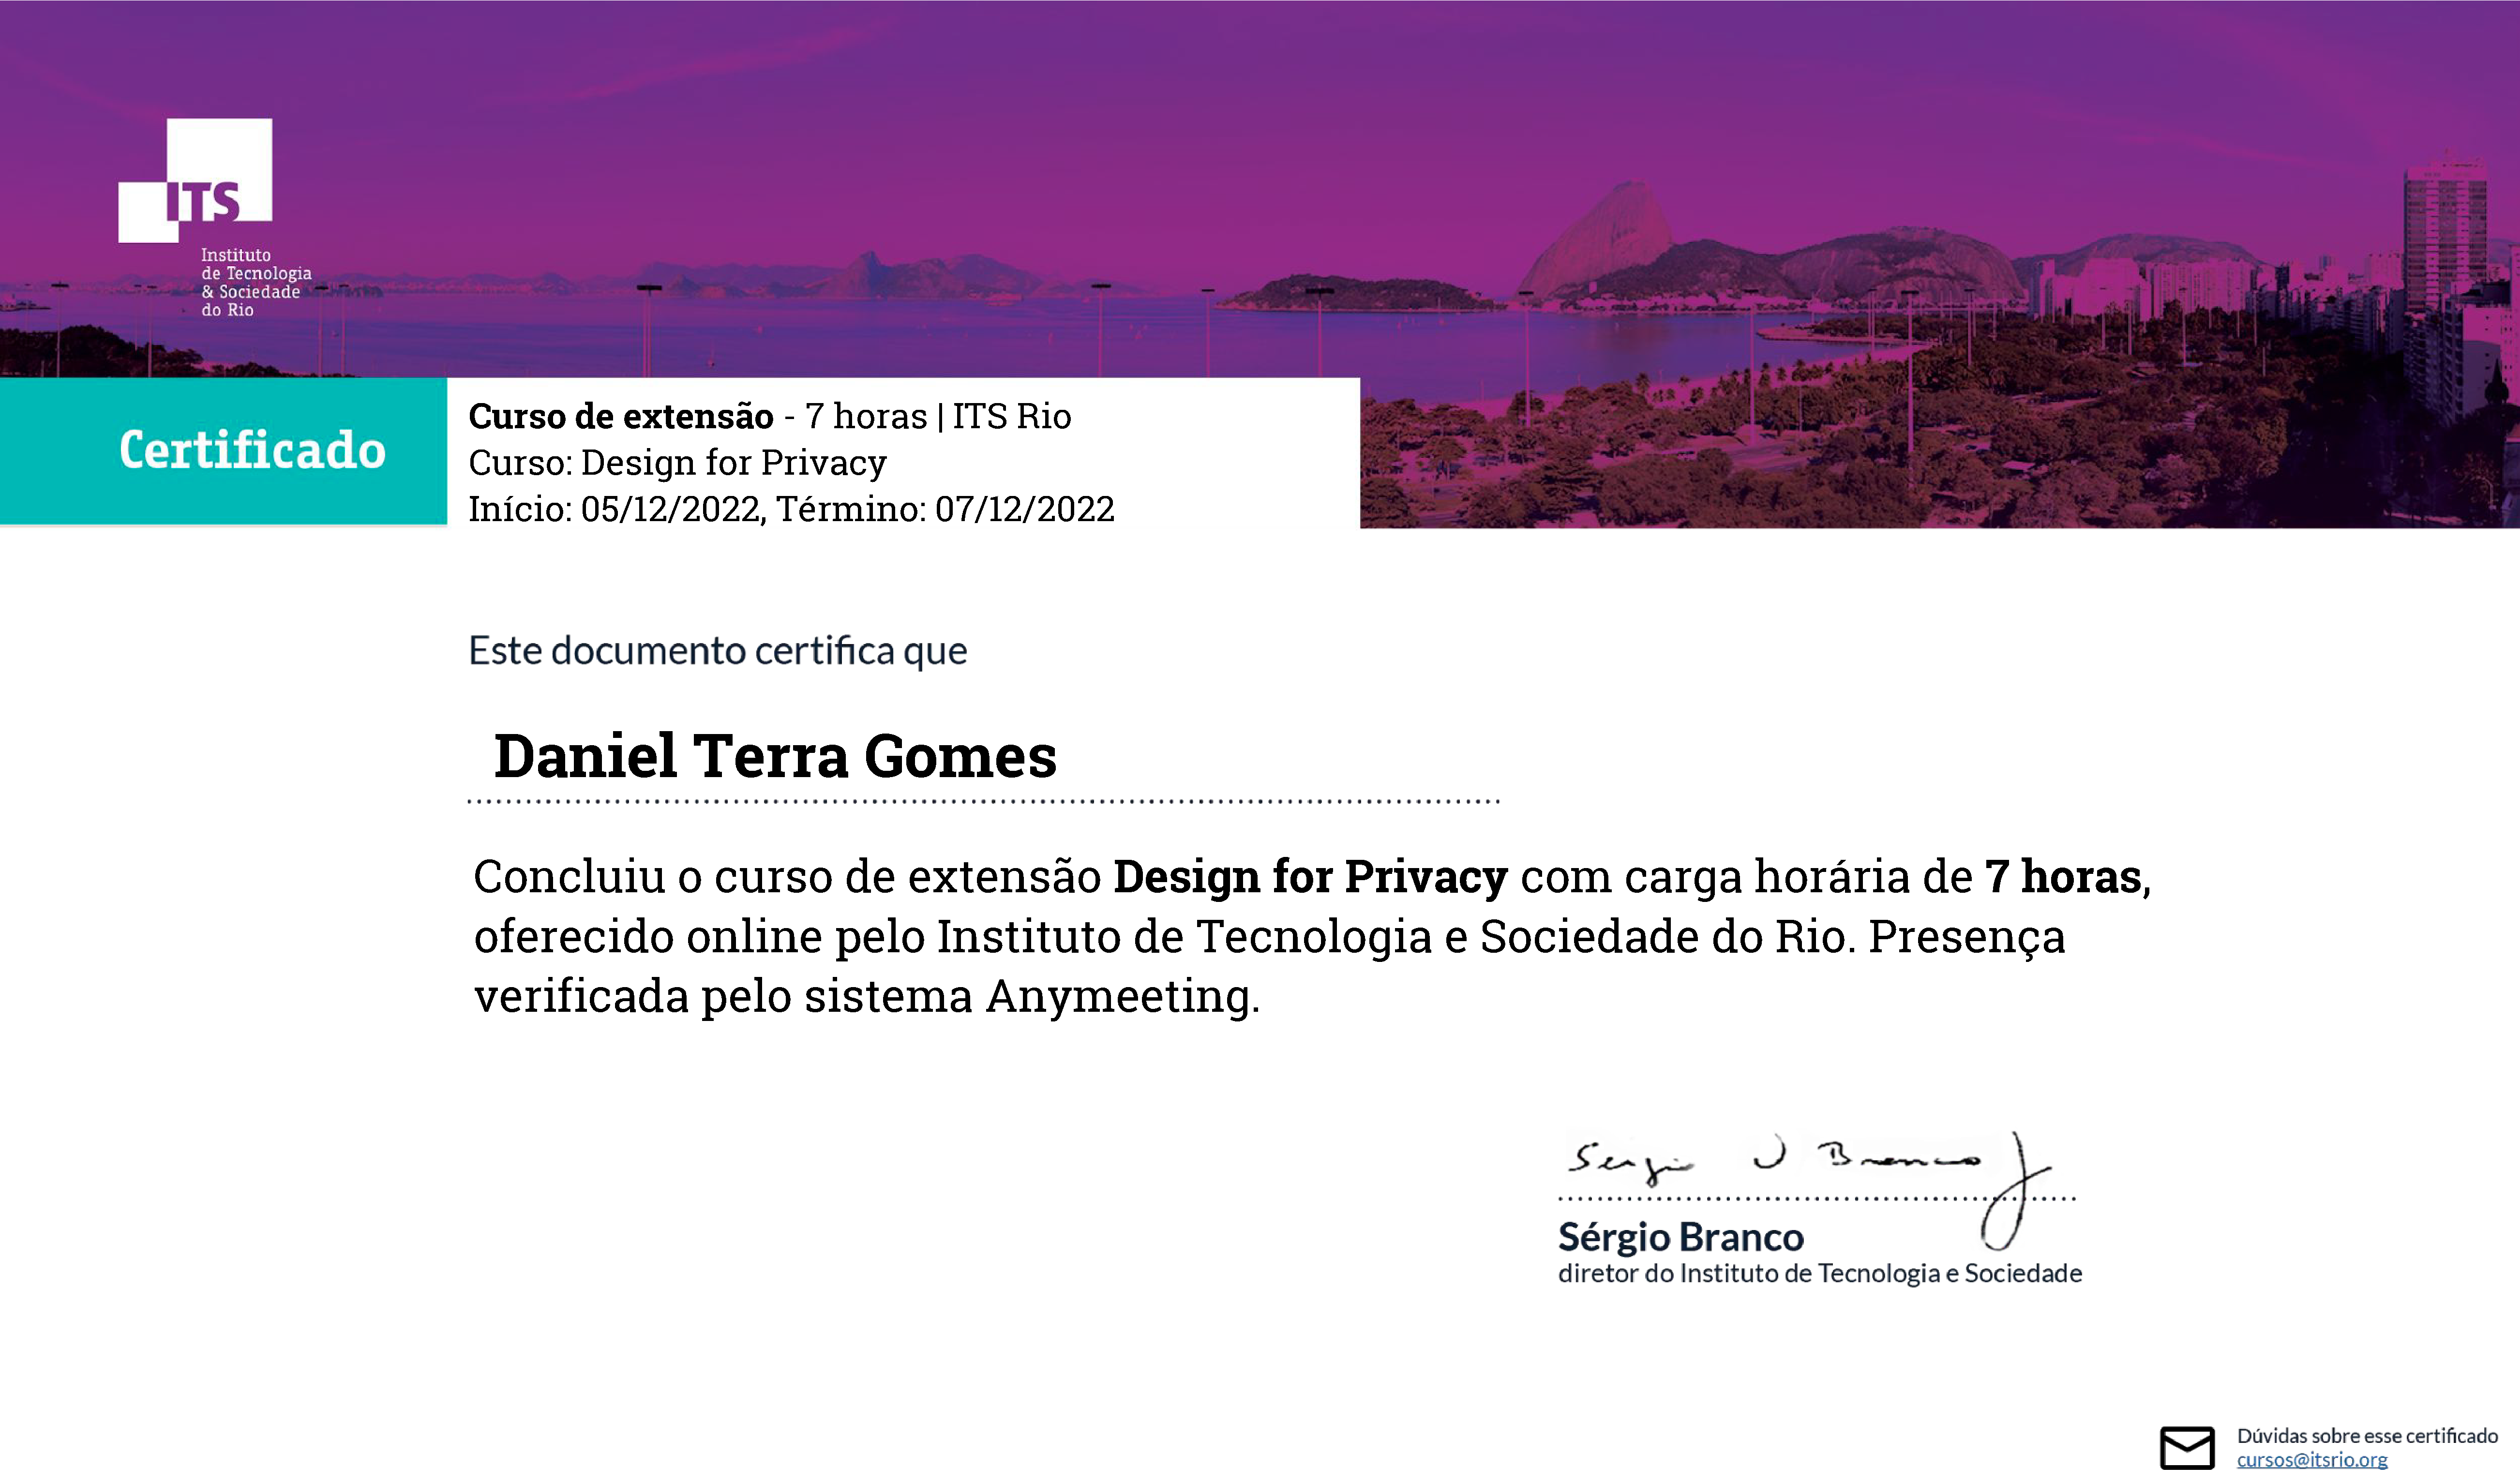
\includegraphics[width=\textwidth]{Figures/its2.pdf}
\caption{Certificado de conclusão ao curso Design for Privacy.}
\label{Direitos}
\end{figure}

\begin{figure}[H]
\centering
    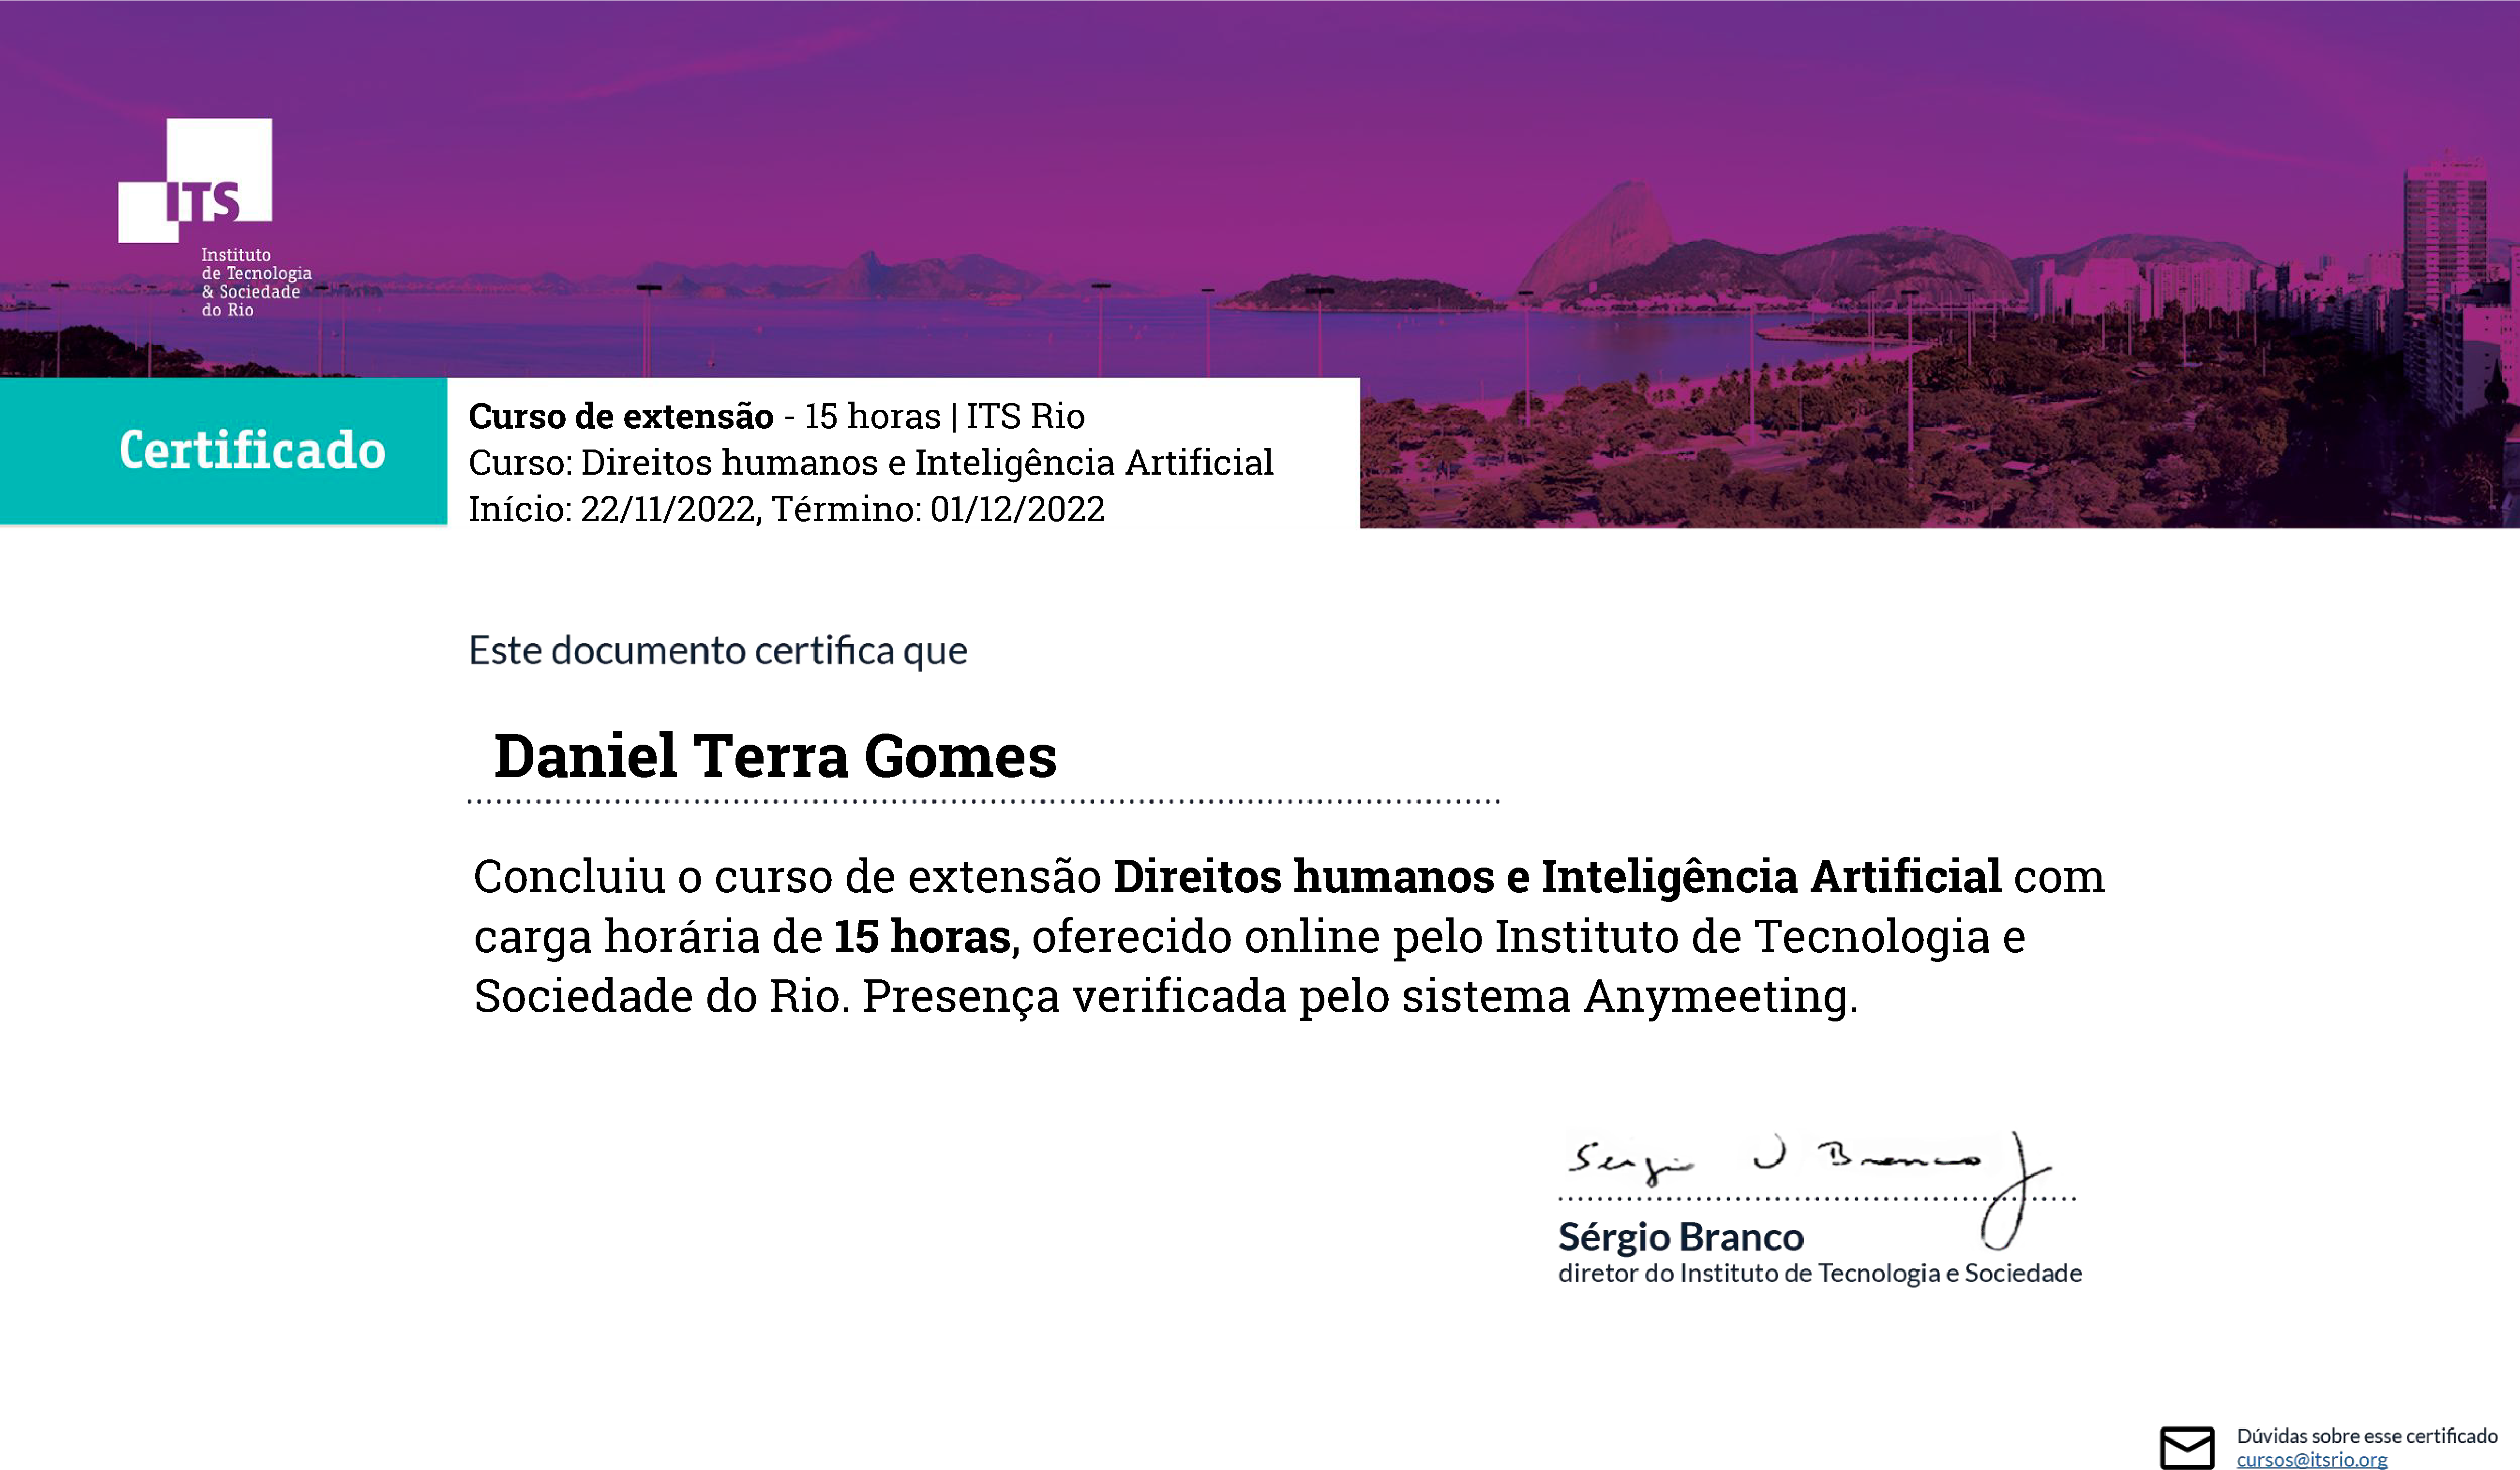
\includegraphics[width=\textwidth]{Figures/its1.pdf}
\caption{Certificado de conclusão ao curso Direitos humanos e Inteligência Artificial.}
\label{Design}
\end{figure}



\chapter{Datas e assinaturas} \label{ass}

\section{Data e assinatura do bolsista (assinatura digitalizada)}


\begin{figure}[H]
 \centering
 
\includegraphics[width=0.4\textwidth]{Figures/sign.png}
 %\caption{\label{kaggle.score}Pontuação final no Kaggle.}
\end{figure}
\center30/04/2023

\section{Data e assinatura do orientador (assinatura digitalizada)}


\begin{figure}[H]
 \centering
 
\includegraphics[width=0.4\textwidth]{Figures/assinatura_annabell.png}
 %\caption{\label{kaggle.score}Pontuação final no Kaggle.}
\end{figure}
\center 30/04/2023

